\documentclass[conference]{IEEEtran}

\usepackage{graphicx}
\usepackage{amsmath,amssymb}
\usepackage{cite}
\usepackage{booktabs}
\usepackage{multirow}
\usepackage{tabularx}
\usepackage{url}
\usepackage{xurl}
\usepackage{pgfplots}
\usepackage{placeins}
\usepackage[hidelinks]{hyperref}
\usepackage[caption=false,font=footnotesize]{subfig}
\pgfplotsset{compat=1.18}

\DeclareMathOperator*{\argmax}{arg\,max}
\DeclareMathOperator{\sgn}{sgn}

% Float placement: pack large floats with surrounding text and avoid near-empty float pages
\renewcommand{\topfraction}{0.95}
\renewcommand{\bottomfraction}{0.85}
\renewcommand{\textfraction}{0.06}
\renewcommand{\floatpagefraction}{0.85}
\renewcommand{\dbltopfraction}{0.95}
\renewcommand{\dblfloatpagefraction}{0.85}
\setcounter{topnumber}{4}
\setcounter{bottomnumber}{3}
\setcounter{totalnumber}{6}
\setcounter{dbltopnumber}{4}

\graphicspath{{./}{./figures/}{./tables/}}

\title{Detection and Risk Assessment of Unsafe Hanging Travel in Public Transport Using Machine Learning}

\author{\IEEEauthorblockN{Tazkia Malik, Sadek Hossain Asif, Tanzila Khan, Taif Ahmed Turjo, Amio Rashid, Mahmud Hasan Walid}
\IEEEauthorblockA{Department of Computer Science and Engineering\\
University of Dhaka\\
Dhaka, Bangladesh}}

\begin{document}
\maketitle

\begin{abstract}
Unsafe door-hanging and overcrowded travel are persistent safety risks in Dhaka's public transport system, particularly in buses and legunas operating under high passenger demand. Existing intelligent transportation research has addressed vehicle detection, passenger counting, and general crowd analysis, but localized automated detection of unsafe hanging travel remains limited. This paper presents an image-based machine-learning framework for classifying public transport scenes into safe/normal and unsafe/risky conditions. A custom bus and leguna image dataset is prepared through cleaning, annotation, preprocessing, and augmentation. For classical machine-learning baselines, Histogram of Oriented Gradients (HOG) descriptors are used with Logistic Regression, Gaussian Naive Bayes, and a Support Vector Machine (SVM) with a radial basis function kernel. Deep models including a CNN trained from scratch, ResNet18, EfficientNet-B0, ResNet50, ConvNeXt-Tiny, and an ensemble are also evaluated to compare learned visual features with handcrafted HOG representations. The retrained dataset contains 523 annotation-labeled images, and augmentation is restricted to the training partition to avoid leakage. On the untouched 79-image test set, the ResNet50--ConvNeXt ensemble reaches 94.7\% unsafe recall, 86.1\% accuracy, and 0.970 ROC-AUC at the balanced operating point, while ResNet50 attains the highest single-model accuracy of 92.4\%. Because a missed hanging passenger is more costly than a false alarm, the system is tuned to favor unsafe-class recall. The results indicate that a localized, annotation-driven dataset with leakage-free augmentation allows standard transfer-learning models to detect unsafe hanging travel with high reliability.
\end{abstract}

\begin{IEEEkeywords}
Unsafe public transport, computer vision, image classification, Histogram of Oriented Gradients, support vector machine, convolutional neural network, intelligent transportation system.
\end{IEEEkeywords}

\section{Introduction}
Public transport in Dhaka carries a large share of daily urban mobility, but high passenger demand, limited vehicle capacity, and inconsistent enforcement often create unsafe conditions. A common visible hazard is door-hanging travel, where passengers ride from the doorway or exterior boundary of buses and legunas, increasing exposure to falls, collisions, and roadside obstacles.

Safety monitoring still depends heavily on traffic personnel, transport operators, or surveillance staff. Manual observation is difficult to scale across dense road networks, heterogeneous vehicle types, and continuously changing traffic scenes.

Computer vision is useful for this task because images can capture vehicle structure, passenger position, crowding, and doorway conditions. This paper proposes an image-based machine-learning system that classifies Dhaka public transport scenes into safe/normal negative samples and unsafe/risky positive samples.

The main contributions are as follows:
\begin{itemize}
    \item A localized safe/unsafe public transport image dataset containing Dhaka bus and leguna scenes.
    \item A complete machine-learning pipeline for unsafe hanging-travel detection.
    \item A comparison of HOG-based classical machine-learning models and deep convolutional models.
    \item An evaluation using standard classification metrics, including accuracy, unsafe-class recall, ROC and precision--recall curves, and AUC, together with a train/validation/test generalization analysis.
\end{itemize}

\section{Related Work}
Computer vision has become an important component of intelligent transportation systems. Surveyed applications include vehicle detection, pedestrian detection, anomaly detection, traffic monitoring, and automatic number-plate recognition \cite{dilek2023cvits}. These methods show that visual data can support automated interpretation of transportation scenes, although most work targets general traffic understanding rather than specific passenger-safety risks.

Passenger monitoring research commonly focuses on counting, occupancy estimation, boarding analysis, and crowd monitoring in buses or terminals \cite{hsu2020passenger}. Public transport safety studies identify overcrowding, weak enforcement, and unsafe passenger behavior as important risk factors in dense urban environments \cite{barua2013brt}, while broader reviews show that crowd pressure and non-collision incidents remain persistent concerns when demand exceeds service capacity \cite{crowding2023review}.

Unsafe behavior and abnormal-activity detection are related to the present task because they aim to identify visual patterns that deviate from normal scenes. Recent surveys report that deep learning can be effective for abnormal behavior detection, but they also emphasize difficulties caused by limited labeled data, occlusion, scene variation, and domain transfer \cite{wastupranata2024abnormal}. Object-detection methods such as YOLO provide another foundation for transportation surveillance and boarding or alighting recognition \cite{redmon2016yolo}, \cite{yolo2024boarding}. Closer to the present task, vision-based systems have been developed to recognize abnormal or unsafe passenger behavior inside buses from onboard cameras \cite{tseng2022bus}, \cite{lin2024bus}, \cite{liu2025bus}, and to analyze passenger posture during the safety-critical boarding and alighting phase at bus doors \cite{ramirez2025posture}. These efforts confirm that onboard and door-region imagery carries strong cues for passenger-safety assessment, but they target in-vehicle activity or door movement rather than passengers hanging from the exterior of a moving vehicle.

Automatic License Plate Recognition (ALPR) is relevant only as future context for identifying vehicles after unsafe behavior is detected. Existing ALPR studies address plate localization and recognition under real-world imaging constraints \cite{anagnostopoulos2008license}, \cite{silva2018license}, \cite{du2013automatic}, including Bengali license-plate recognition under low-resolution and blurred conditions \cite{afrin2023bengali}.

The key gap is that existing work rarely addresses unsafe door-hanging detection in Dhaka-like crowded public transport environments using localized datasets under real-world challenges such as occlusion, motion blur, lighting variation, crowding, and non-standard vehicle structures. Prior systems often estimate occupancy, count passengers, or recognize boarding events, but they do not directly model hanging passengers as a safety-critical positive class under local bus and leguna conditions. Safety interventions for footboard travel in South Asian buses have relied mainly on onboard IoT sensors rather than vision \cite{indhumathi2024footboard}, and although localized Bangladeshi image datasets exist for vehicle-type classification \cite{tabassum2020poribohon}, none label unsafe door-hanging behavior.

\section{Dataset}
\subsection{Data Collection}
The dataset contains images of buses and legunas captured under real-world public transport conditions in Dhaka. The samples cover safe/normal and unsafe/risky cases with variation in vehicle type, passenger density, camera angle, lighting, and scene clutter. Labels are derived from image annotations: an image is unsafe if it contains at least one box labeled \texttt{unsafe}; otherwise it is safe, and license-plate boxes are ignored. The retrained dataset contains 523 labeled originals, with 272 safe samples and 251 unsafe samples. Figure~\ref{fig:eda} summarizes the updated class distribution and split composition, and Table~\ref{tab:dataset_composition} lists the per-partition counts.

\begin{figure}[!t]
    \centering
    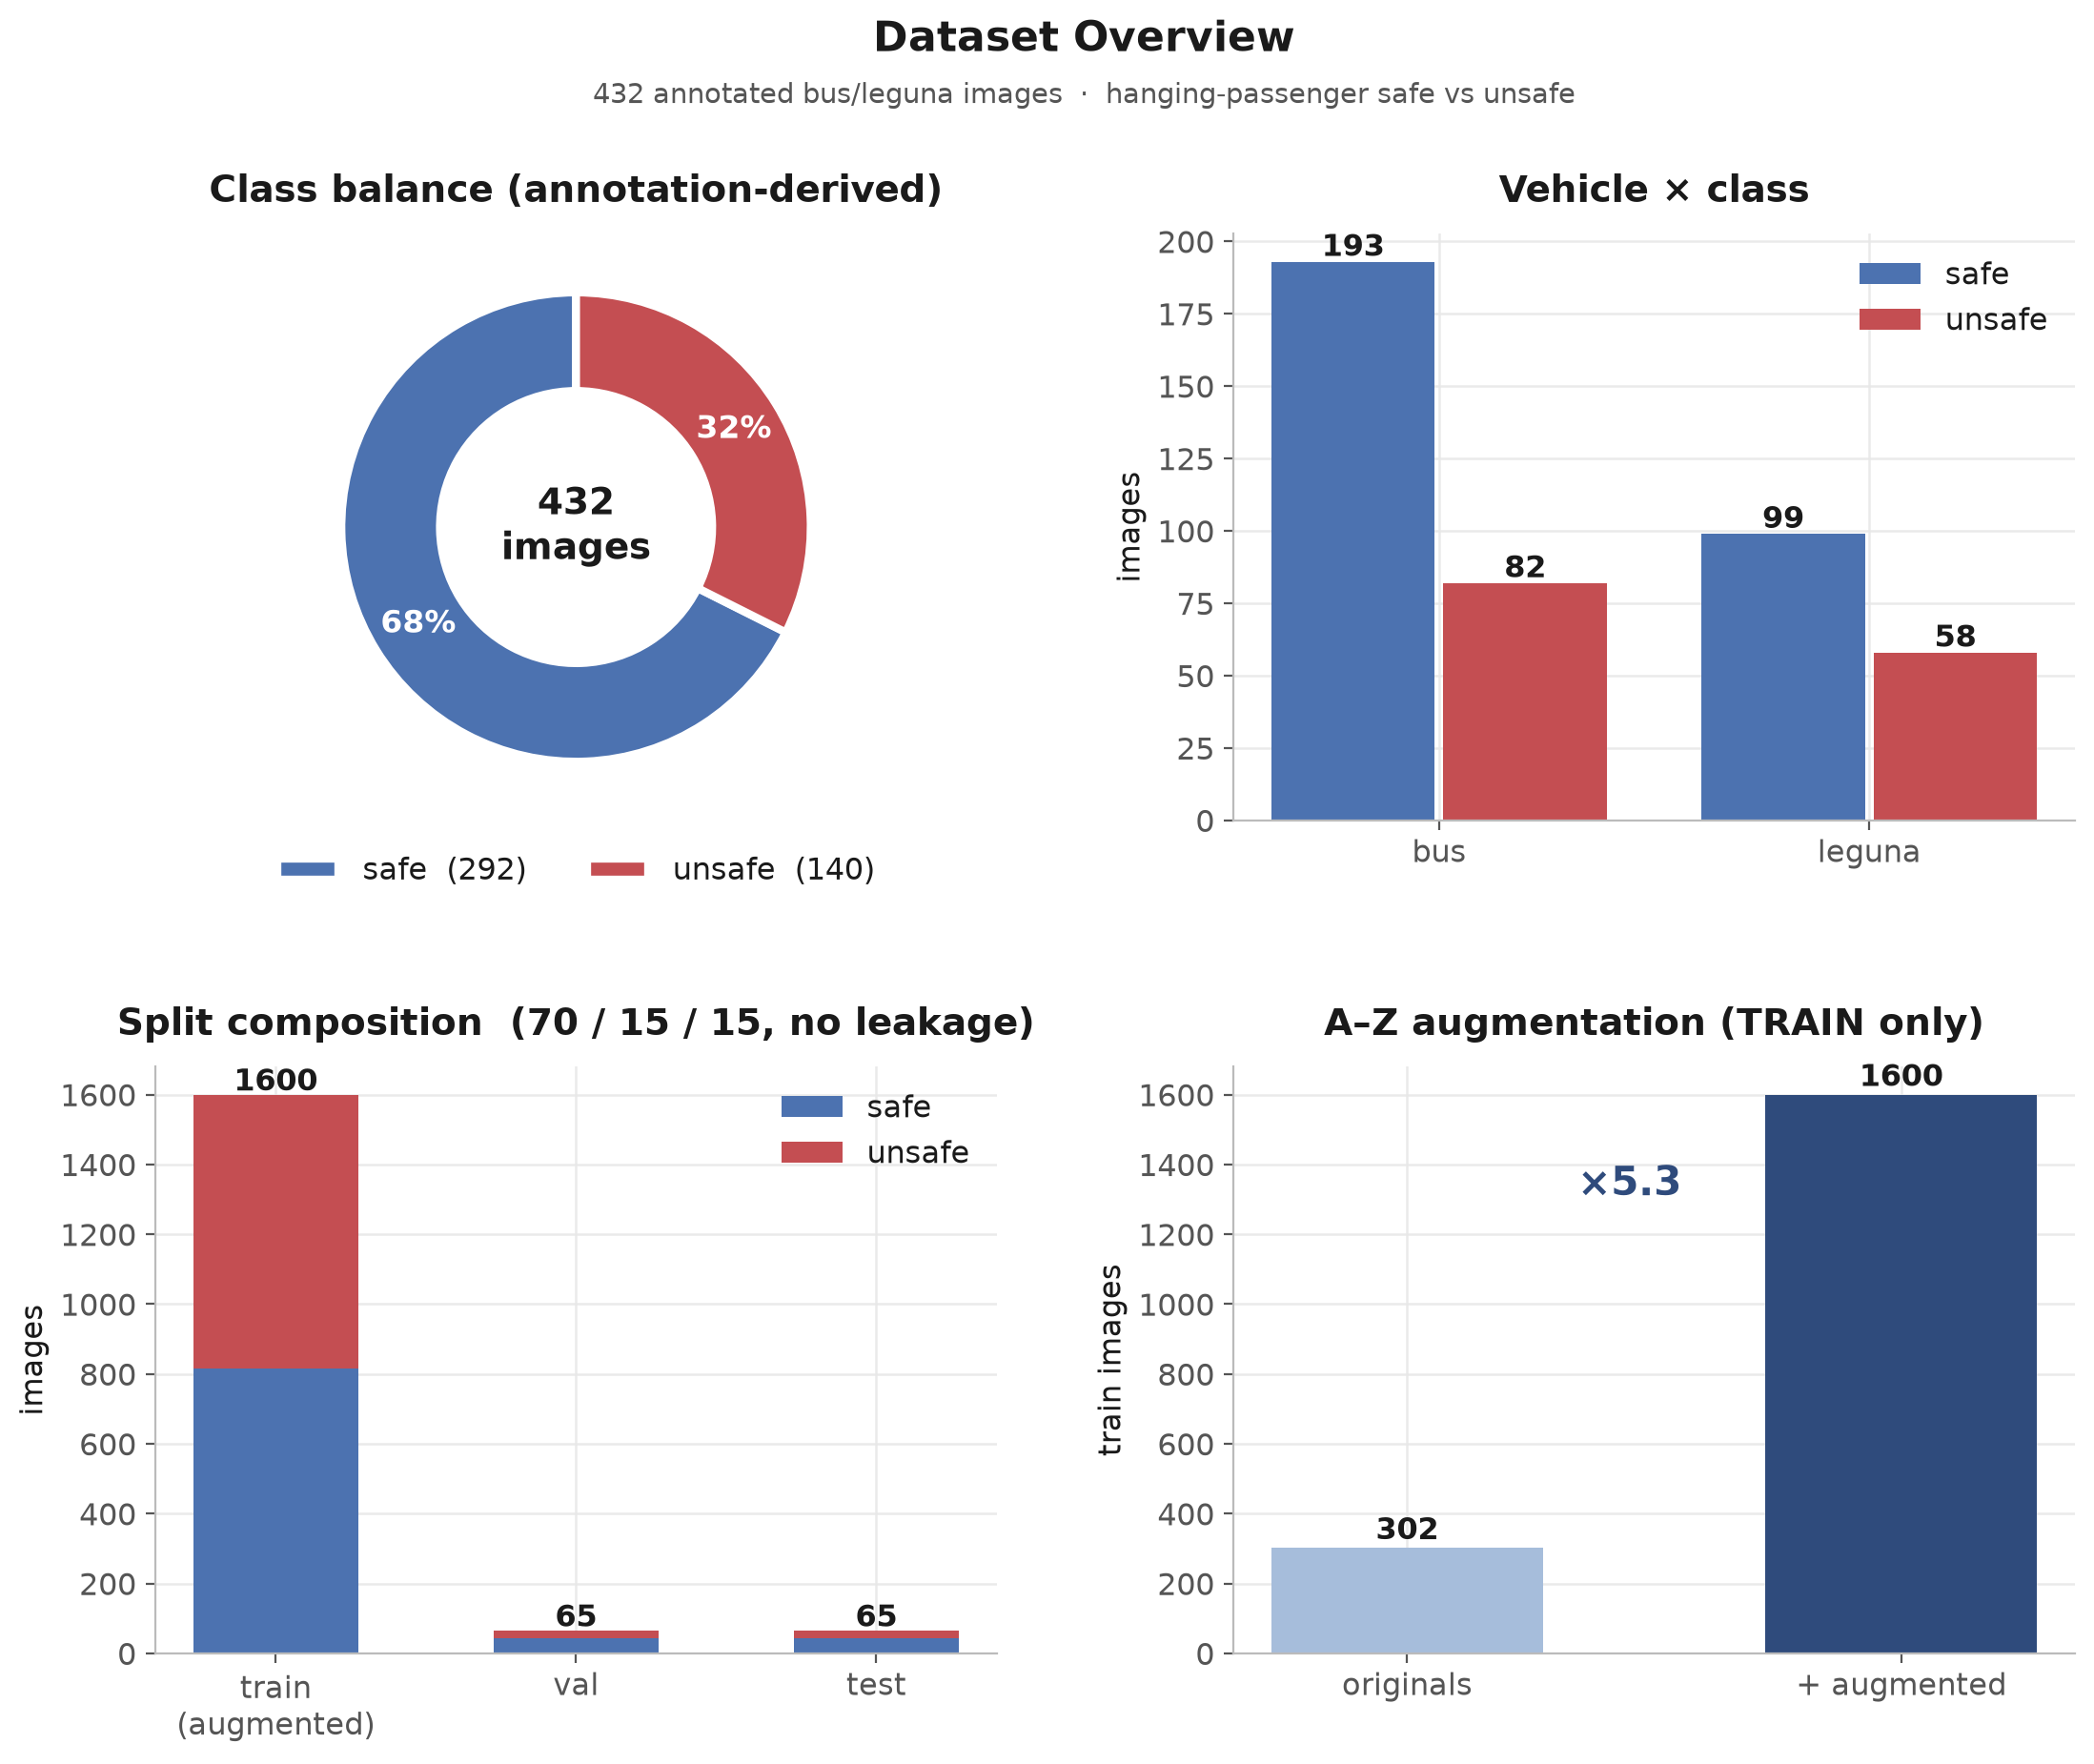
\includegraphics[width=\linewidth]{figures/fig01_dataset_overview.png}
    \caption{Dataset overview: annotation-derived class balance, vehicle-wise class distribution across buses and legunas, stratified 70/15/15 split composition, and train-only augmentation growth from 365 originals to 2{,}730 training images.}
    \label{fig:eda}
\end{figure}

\begin{table}[!t]
\centering
\caption{Dataset Composition After Splitting and Train-Only Augmentation}
\label{tab:dataset_composition}
\footnotesize
\setlength{\tabcolsep}{5pt}
\begin{tabular}{lrrr}
\toprule
\textbf{Partition} & \textbf{Total} & \textbf{Safe} & \textbf{Unsafe} \\
\midrule
Training (augmented) & 2{,}730 & 1{,}330 & 1{,}400 \\
Validation & 79 & 41 & 38 \\
Test & 79 & 41 & 38 \\
Labeled originals & 523 & 272 & 251 \\
\bottomrule
\end{tabular}
\end{table}

Representative examples of the vehicle categories are shown in Fig.~\ref{fig:leguna_samples} and Fig.~\ref{fig:bus_samples}.

\begin{figure}[!t]
    \centering
    \subfloat[Negative class.]{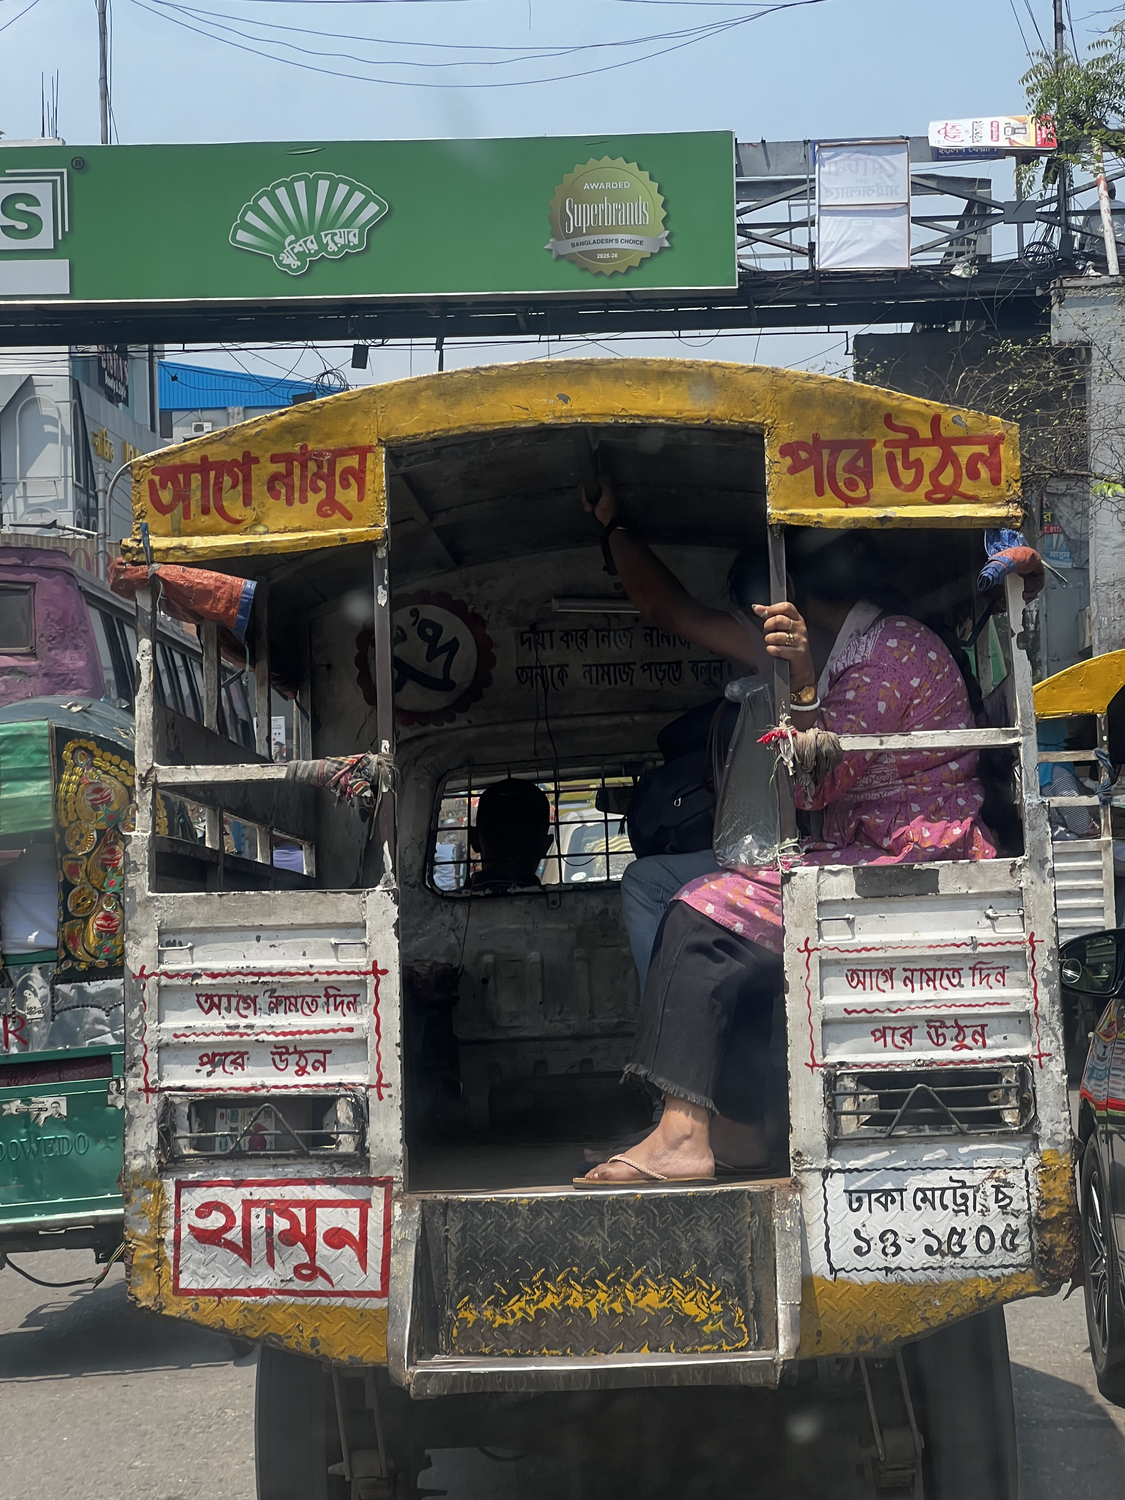
\includegraphics[width=0.4\linewidth]{leguna_negative.png}}
    \hfill
    \subfloat[Positive class.]{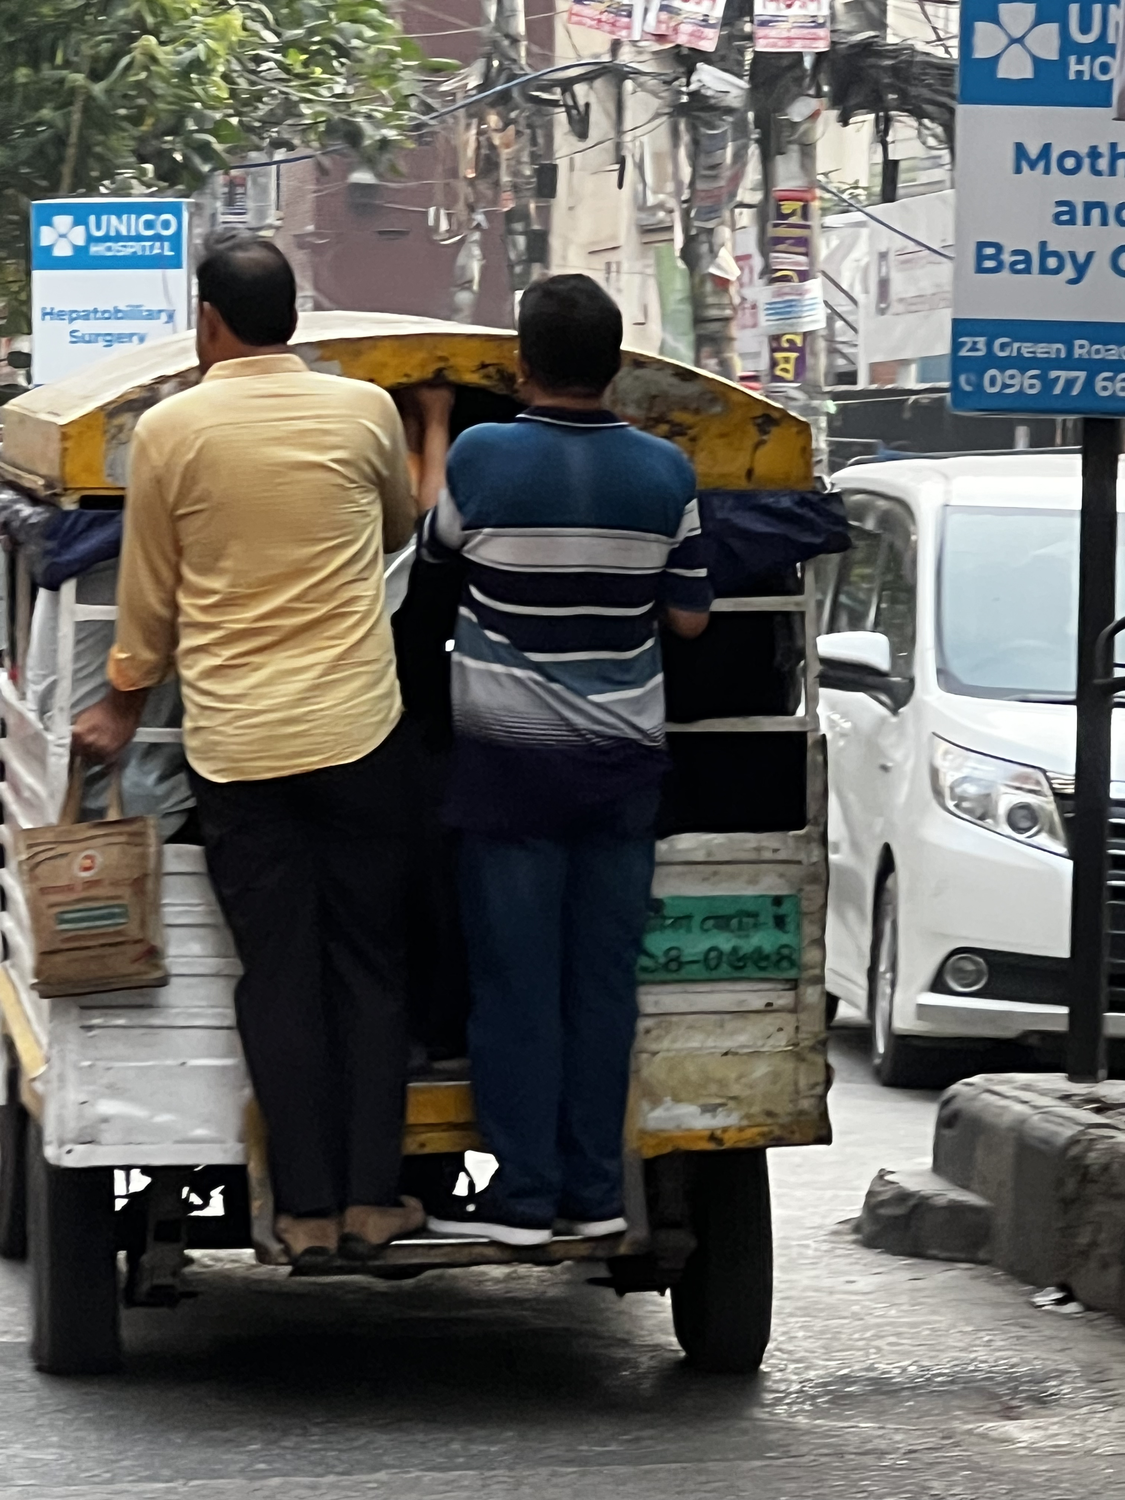
\includegraphics[width=0.4\linewidth]{leguna_positive.png}}
    \caption{Representative leguna samples.}
    \label{fig:leguna_samples}
\end{figure}

\begin{figure}[!t]
    \centering
    \subfloat[Negative class.]{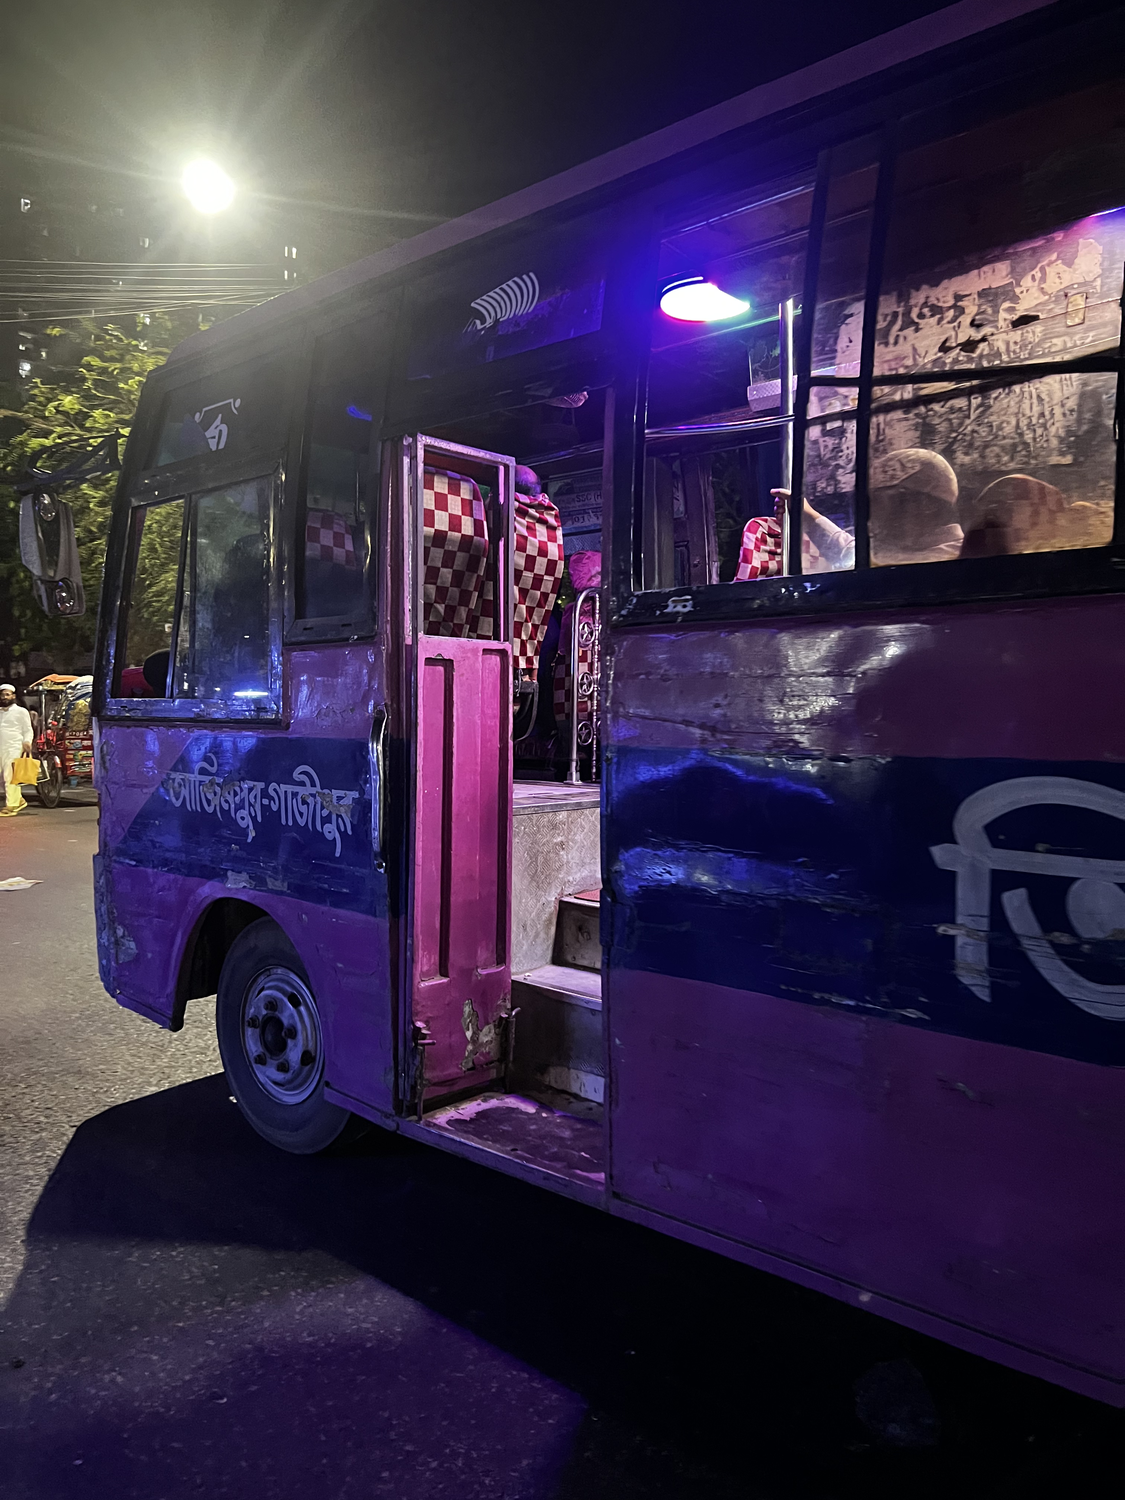
\includegraphics[width=0.4\linewidth]{bus_negative.png}}
    \hfill
    \subfloat[Positive class.]{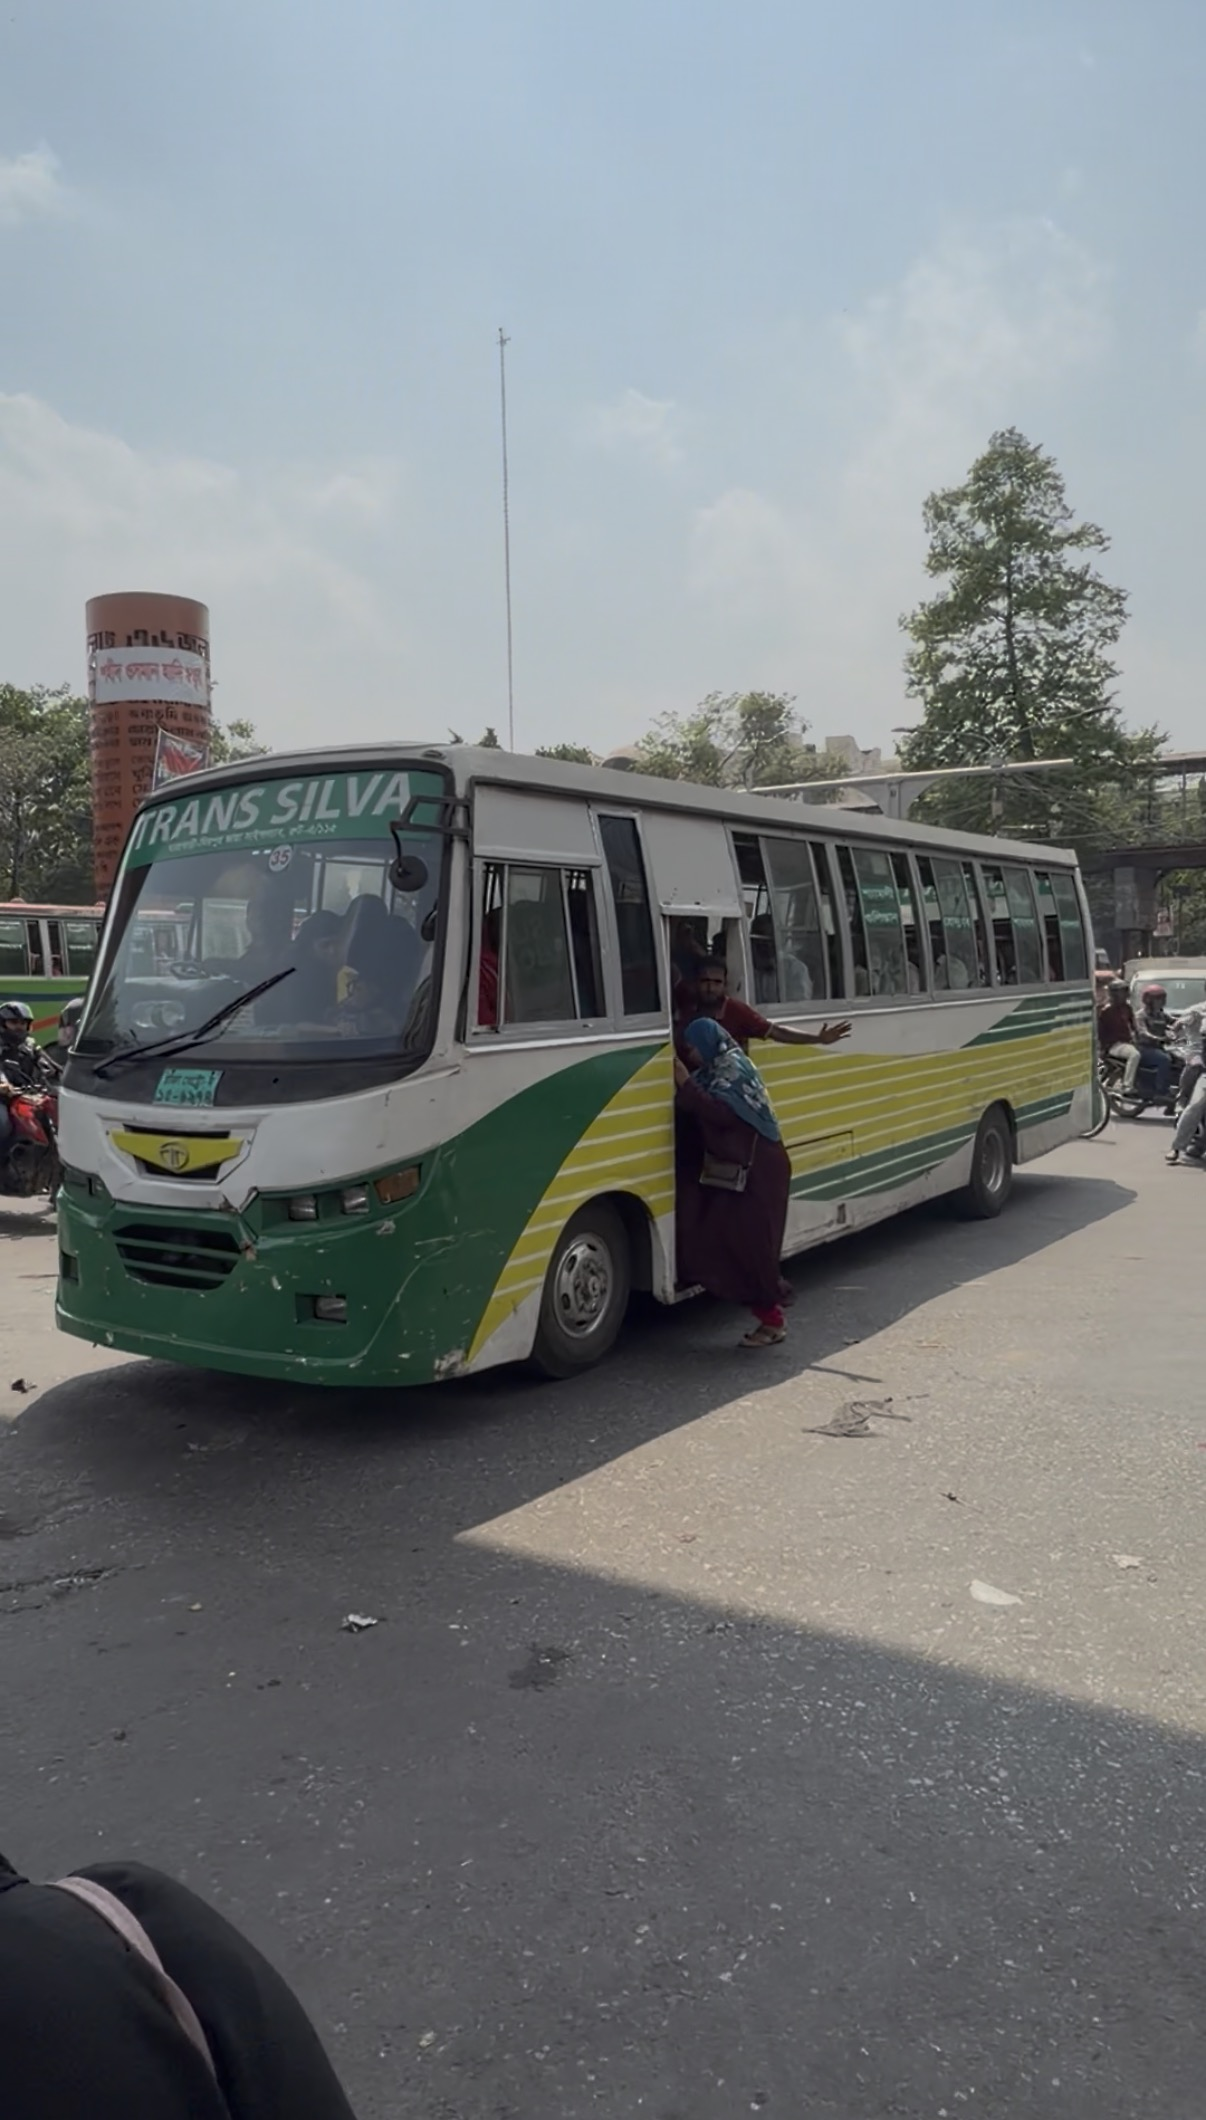
\includegraphics[width=0.4\linewidth]{bus_positive.png}}
    \caption{Representative bus samples.}
    \label{fig:bus_samples}
\end{figure}

\subsection{Data Cleaning}
Cleaning removed images whose content was blurred, ambiguous, low quality, heavily obstructed, poorly framed, or unreliable for class assignment. This step reduced label noise while preserving realistic variation in traffic, vehicle structure, crowding, and illumination.

\subsection{Data Annotation}
Manual annotation assigned each retained image to one of two classes: negative for safe/normal passenger conditions and positive for unsafe/risky hanging travel. Figure~\ref{fig:annotation_samples} shows representative annotation examples.

\begin{figure}[!t]
    \centering
    \subfloat[Unsafe/risky annotation.]{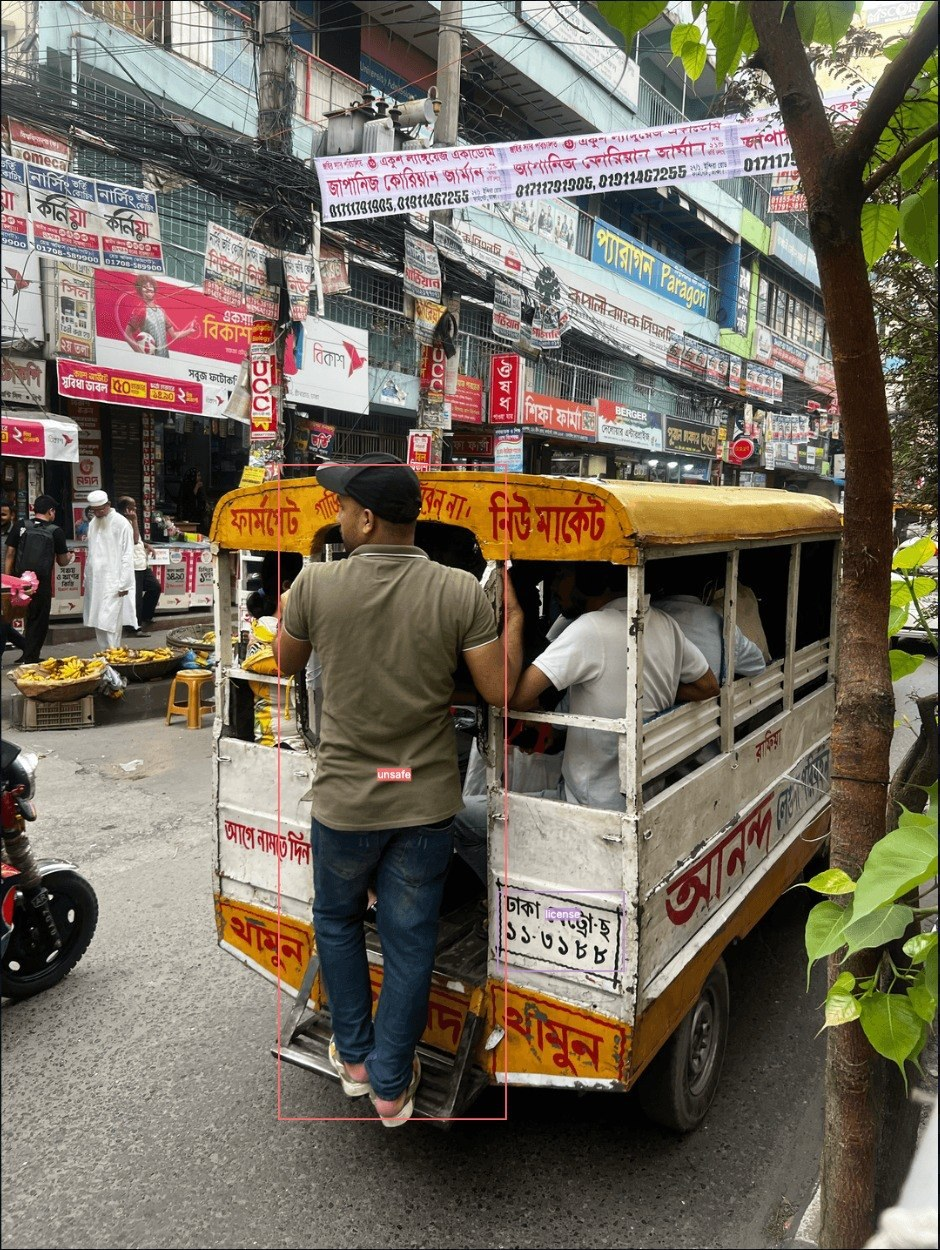
\includegraphics[width=0.35\linewidth]{annotation_1.jpeg}}
    \hfill
    \subfloat[Safe/normal annotation.]{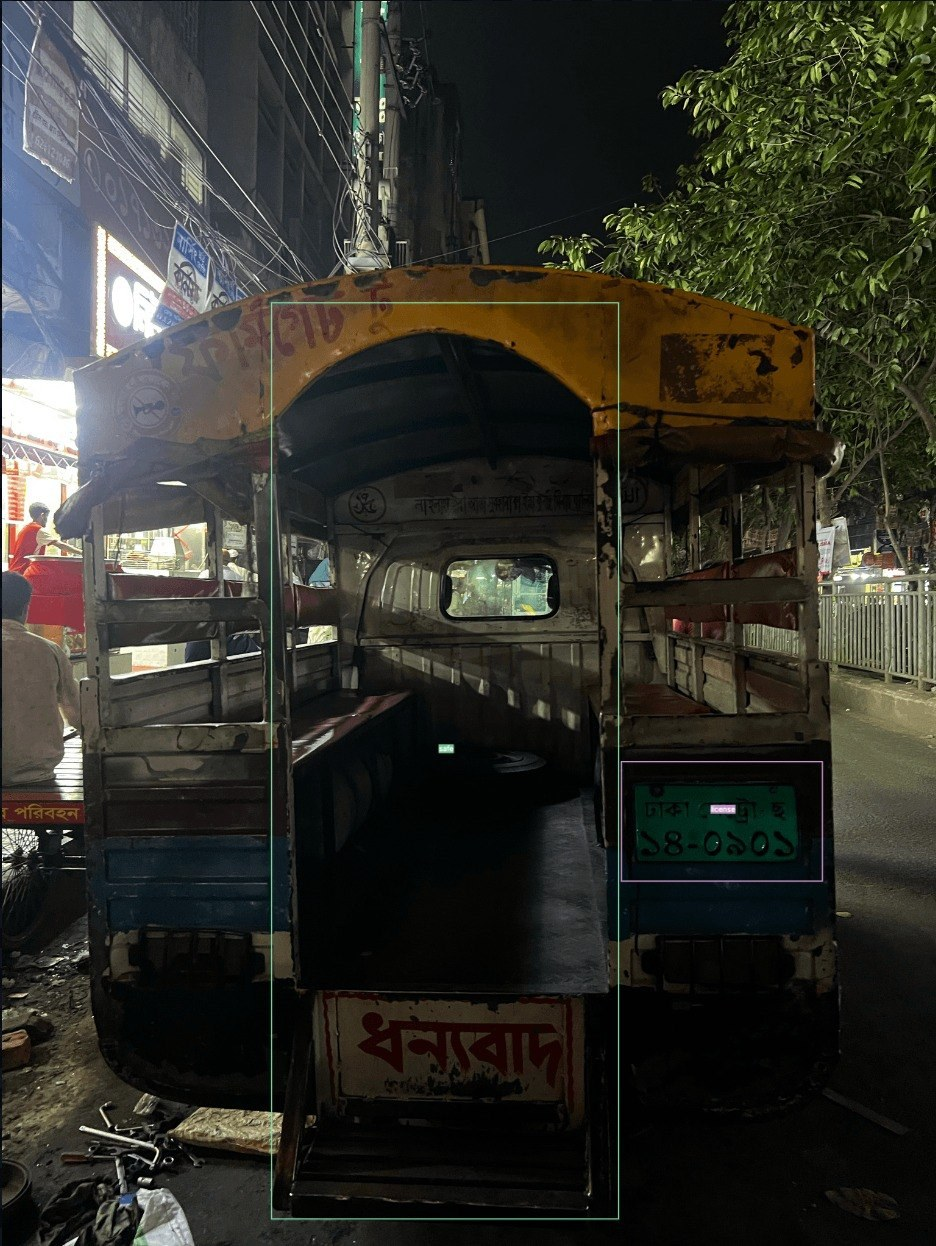
\includegraphics[width=0.35\linewidth]{annotation_2.jpeg}}
    \caption{Representative annotation examples.}
    \label{fig:annotation_samples}
\end{figure}

\subsection{Data Augmentation}
Augmentation was restricted to the training partition to prevent leakage into validation or test data. The 365 training originals produced 2,365 offline augmented samples, yielding 2,730 training images with 1,330 safe and 1,400 unsafe samples. Validation and test each contain 79 unaugmented originals, divided into 41 safe and 38 unsafe images. Deep models additionally used online augmentation, weighted sampling, and horizontal-flip test-time augmentation. These transformations simulate common roadside imaging variation while preserving the class label \cite{shorten2019augmentation}.

All images were standardized before model-specific processing. The standardized preprocessing and model input settings are summarized in Table~\ref{tab:model_config}. The dataset is available online at \url{https://drive.google.com/drive/folders/1D3jDBvA-cAhwRPA4wUBUss5zlwdXdLJY}.

\subsection{Ethical Considerations}
The dataset is used only for academic safety-monitoring research. Images may contain privacy-sensitive visual information such as human faces, vehicle license plates, and location-related context. The classification task focuses on transport safety conditions rather than personal identity recognition; no face recognition, identity matching, or individual profiling is performed. Before any public release or operational deployment, privacy-preserving steps such as face and license-plate anonymization, removal of GPS or location metadata, consent and data-governance procedures, and compliance with relevant regulations would be required.

\section{Methodology}
The proposed method is a binary image-classification pipeline for public transport safety assessment. The workflow consists of dataset preparation, preprocessing, feature extraction or model-specific input preparation, model training, and evaluation. HOG-based classical models receive handcrafted gradient features, while deep neural models learn directly from image tensors. Implementation settings are summarized in Table~\ref{tab:model_config}.

\subsection{Pipeline Overview}
The pipeline begins with Dhaka bus and leguna image collection, followed by cleaning, annotation, augmentation, and standardization. Classical machine-learning models use HOG feature vectors extracted from grayscale inputs, whereas CNN and transfer-learning models receive RGB tensors. All models are evaluated on the same held-out split using standard classification metrics.

\subsection{Training and Inference Procedure}
The complete retraining procedure is summarized below so that data preparation, model fitting, and deployment decisions are defined within the methodology.
\begin{enumerate}
    \item \textbf{Annotation-based labeling:} Begin with 523 labeled originals containing 272 safe and 251 unsafe images. Assign an image to the unsafe class when at least one annotation box is labeled \texttt{unsafe}; ignore license-plate boxes.
    \item \textbf{Four-way stratification:} Split the originals 70/15/15 over vehicle type and class, preserving bus-safe, bus-unsafe, leguna-safe, and leguna-unsafe samples in validation and test partitions.
    \item \textbf{Leakage-free augmentation:} Apply offline augmentation only to the 365 training originals, producing 2,730 training images. Keep the 79-image validation and 79-image test partitions unaugmented.
    \item \textbf{Model-specific preparation:} Extract standardized HOG features followed by PCA for classical models. Supply normalized RGB tensors to the scratch CNN and ImageNet-pretrained transfer-learning models.
    \item \textbf{Model training:} Train Logistic Regression, Gaussian Naive Bayes, SVM, and the scratch CNN as baselines. Fine-tune ResNet18, EfficientNet-B0, ResNet50, and ConvNeXt-Tiny in two phases. Use weighted sampling and class-weighted loss for deep models.
    \item \textbf{Validation and ensembling:} Tune balanced, high-recall, and max-recall decision thresholds on validation predictions. Form the final ensemble by averaging ResNet50 and ConvNeXt-Tiny unsafe-class probabilities.
    \item \textbf{Test-time inference:} Apply horizontal-flip test-time augmentation to the deep models, average the resulting probabilities, select the configured operating threshold, and evaluate once on the untouched test set.
\end{enumerate}

\begin{figure}[!t]
    \centering
    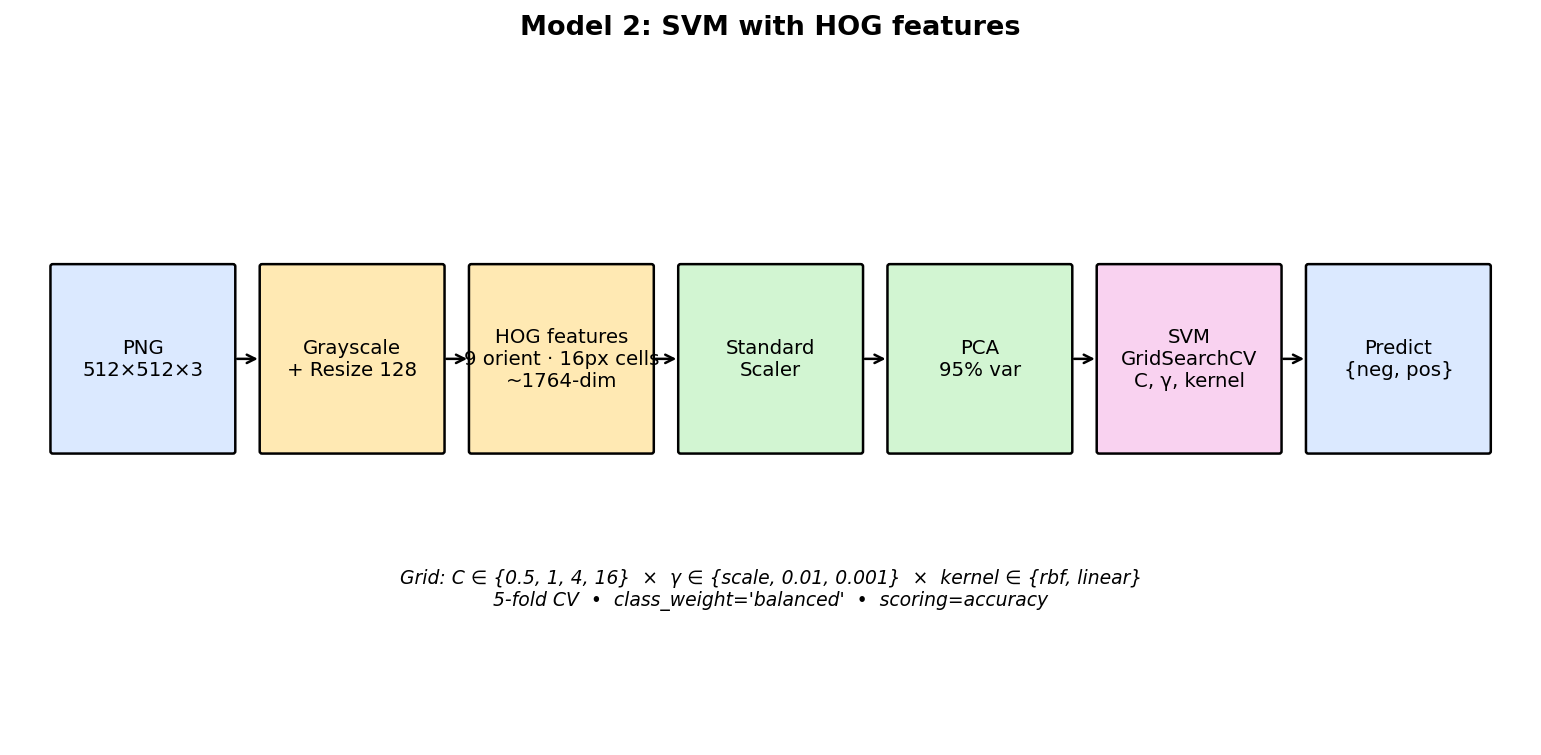
\includegraphics[width=\linewidth]{arch_svm.png}
    \caption{Overview of the HOG-based classical machine-learning pipeline.}
    \label{fig:arch_svm}
\end{figure}

\subsection{HOG-Based Feature Representation}
For the classical models, Histogram of Oriented Gradients (HOG) descriptors were extracted from grayscale images \cite{dalal2005hog}. HOG captures local gradient orientation and edge-structure information, which is useful for posture-, shape-, and boundary-related visual classification. Feature extraction was implemented with scikit-image \cite{vanderwalt2014skimage}; Table~\ref{tab:model_config} lists the extraction settings, and Fig.~\ref{fig:arch_svm} shows the full classical pipeline.

\subsection{Classical Machine Learning Models}
The classical baselines use HOG features with three complementary classifiers. Logistic Regression provides a linear probabilistic baseline and estimates the posterior probability of the positive (unsafe) class as
\begin{equation}
P(y = 1 \mid \mathbf{x}) = \sigma\!\left(\mathbf{w}^{\top}\mathbf{x} + b\right)
= \frac{1}{1 + \exp\!\left(-(\mathbf{w}^{\top}\mathbf{x} + b)\right)},
\end{equation}
where $\mathbf{x} \in \mathbb{R}^{d}$ is the PCA-reduced HOG feature vector, $\mathbf{w} \in \mathbb{R}^{d}$ and $b \in \mathbb{R}$ are the learned weight vector and bias, and $\sigma(\cdot)$ is the logistic sigmoid. The model is computationally efficient and interpretable, but its linear decision boundary can be limited when safe and unsafe samples are not linearly separable.

Gaussian Naive Bayes is a probabilistic baseline that assumes conditional independence among features given the class label. Each feature $x_i$ is modeled with a class-conditional Gaussian likelihood,
\begin{equation}
\begin{split}
p(x_i \mid y) &= \mathcal{N}\!\left(x_i;\, \mu_{y,i},\, \sigma_{y,i}^{2}\right) \\
&= \frac{1}{\sqrt{2\pi\,\sigma_{y,i}^{2}}}\,
\exp\!\left(-\frac{(x_i - \mu_{y,i})^{2}}{2\,\sigma_{y,i}^{2}}\right),
\end{split}
\end{equation}
where $\mu_{y,i}$ and $\sigma_{y,i}^{2}$ are the mean and variance of feature $i$ under class $y$. Assuming conditional independence, the predicted label maximizes the class posterior,
\begin{equation}
\hat{y} = \argmax_{y \in \{0, 1\}} \; P(y) \prod_{i=1}^{d} p(x_i \mid y).
\end{equation}
Although the independence assumption is restrictive for correlated HOG features, the model is useful as a low-complexity comparator.

The Support Vector Machine (SVM) seeks a maximum-margin boundary between the negative and positive classes \cite{cortes1995svm}. To model non-linear separation in the HOG feature space, the radial basis function (RBF) kernel measures the similarity between two feature vectors,
\begin{equation}
K(\mathbf{x}_i, \mathbf{x}_j) = \exp\!\left(-\gamma\, \lVert \mathbf{x}_i - \mathbf{x}_j \rVert_2^{2}\right), \qquad \gamma > 0,
\end{equation}
and the decision function for a test vector $\mathbf{x}$ is
\begin{equation}
f(\mathbf{x}) = \sgn\!\left(\sum_{i \in \mathcal{S}} \alpha_i\, y_i\, K(\mathbf{x}_i, \mathbf{x}) + b\right),
\end{equation}
where $\mathcal{S}$ indexes the support vectors, $\alpha_i \ge 0$ are the learned dual coefficients, $y_i \in \{-1, +1\}$ are the training labels, and $b$ is the bias. The penalty $C$, kernel width $\gamma$, and kernel type were selected by five-fold grid search on the training data. Table~\ref{tab:model_config} summarizes the implementation settings for all three classical models.

\subsection{Deep Neural Models}
The deep models process RGB images directly and learn spatial features from the training data \cite{krizhevsky2012alexnet}. The experiments evaluate five neural architectures: a CNN trained from scratch, ResNet18, EfficientNet-B0, ResNet50, and ConvNeXt-Tiny. The scratch CNN provides a lightweight learned-feature baseline, while the other architectures use ImageNet-pretrained weights and two-phase fine-tuning \cite{he2016resnet}, \cite{tan2019efficientnet}, \cite{liu2022convnext}. A probability-level ensemble combines ResNet50 and ConvNeXt-Tiny. All neural models use batch normalization \cite{ioffe2015batchnorm} for stable optimization and dropout \cite{srivastava2014dropout} for regularization. Weighted sampling, class-weighted loss, validation-tuned thresholds, and horizontal-flip test-time augmentation address imbalance and improve unsafe-class recall. Figure~\ref{fig:arch_cnn} shows the scratch CNN architecture and Fig.~\ref{fig:arch_resnet} illustrates the two-phase transfer-learning scheme shared by the pretrained models; Table~\ref{tab:model_config} reports the combined configuration.

\begin{figure}[!t]
    \centering
    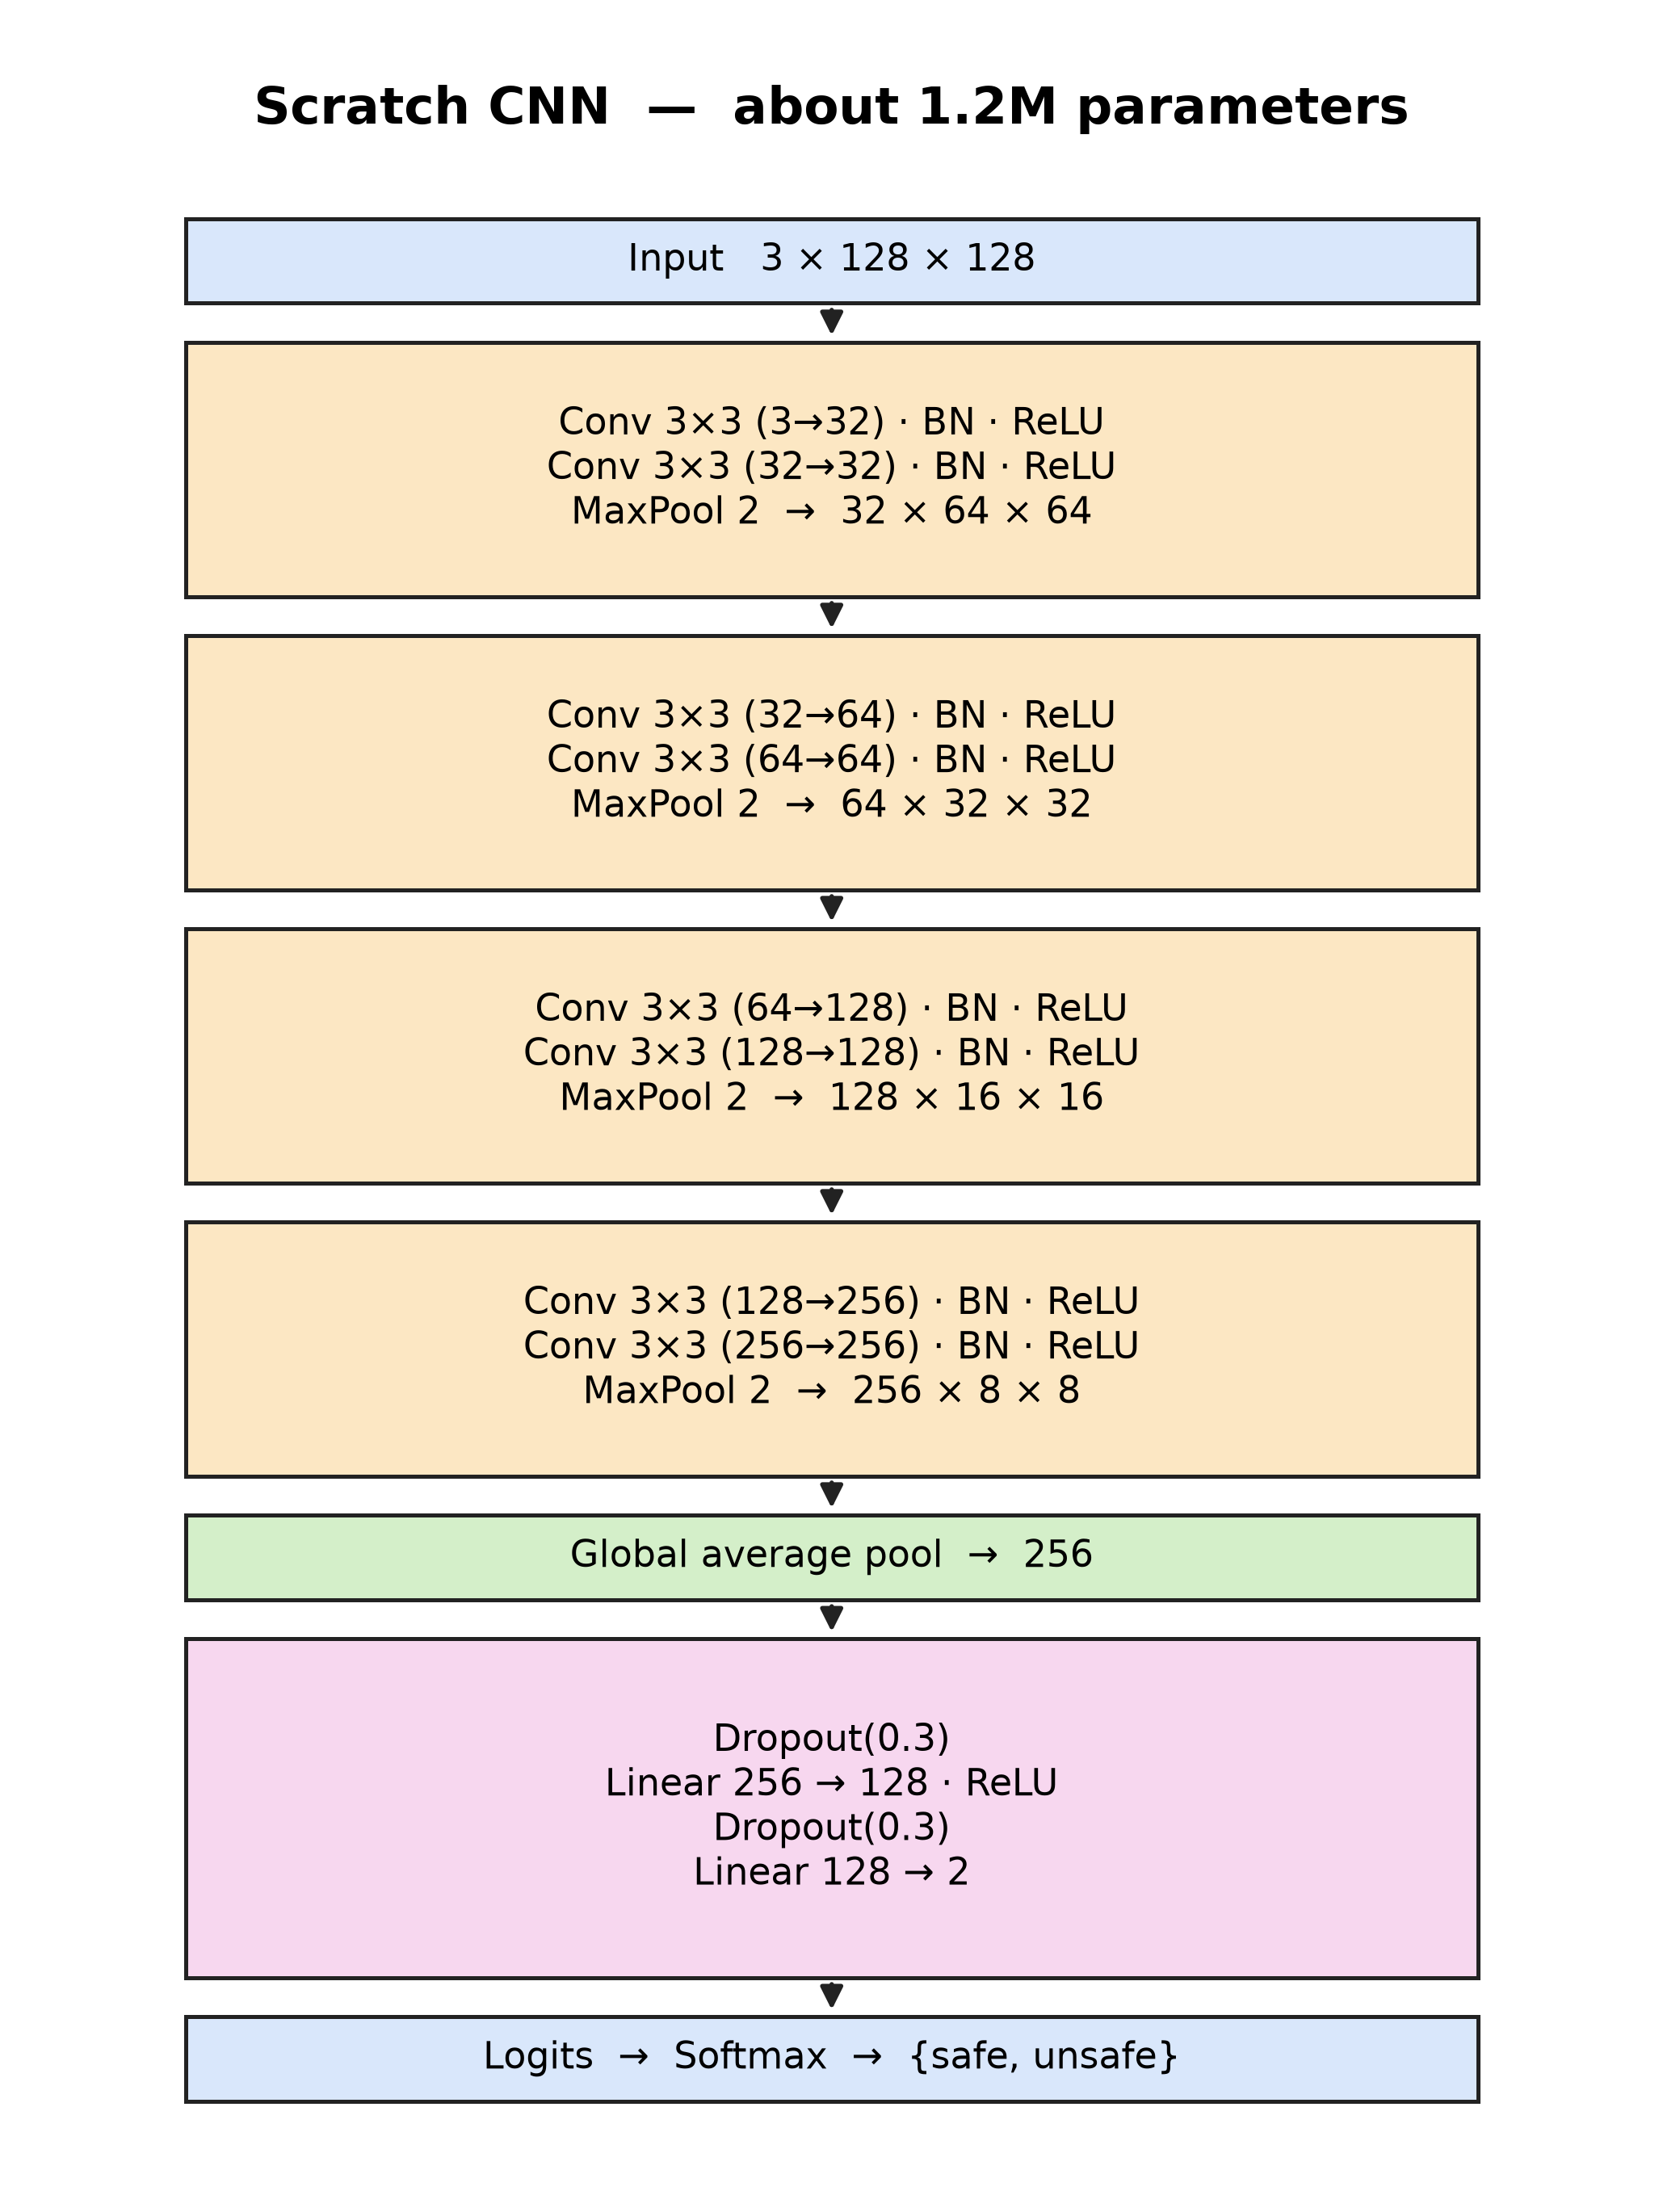
\includegraphics[width=\linewidth]{arch_cnn.png}
    \caption{Scratch CNN architecture used for image-level binary classification.}
    \label{fig:arch_cnn}
\end{figure}

\begin{figure}[!t]
    \centering
    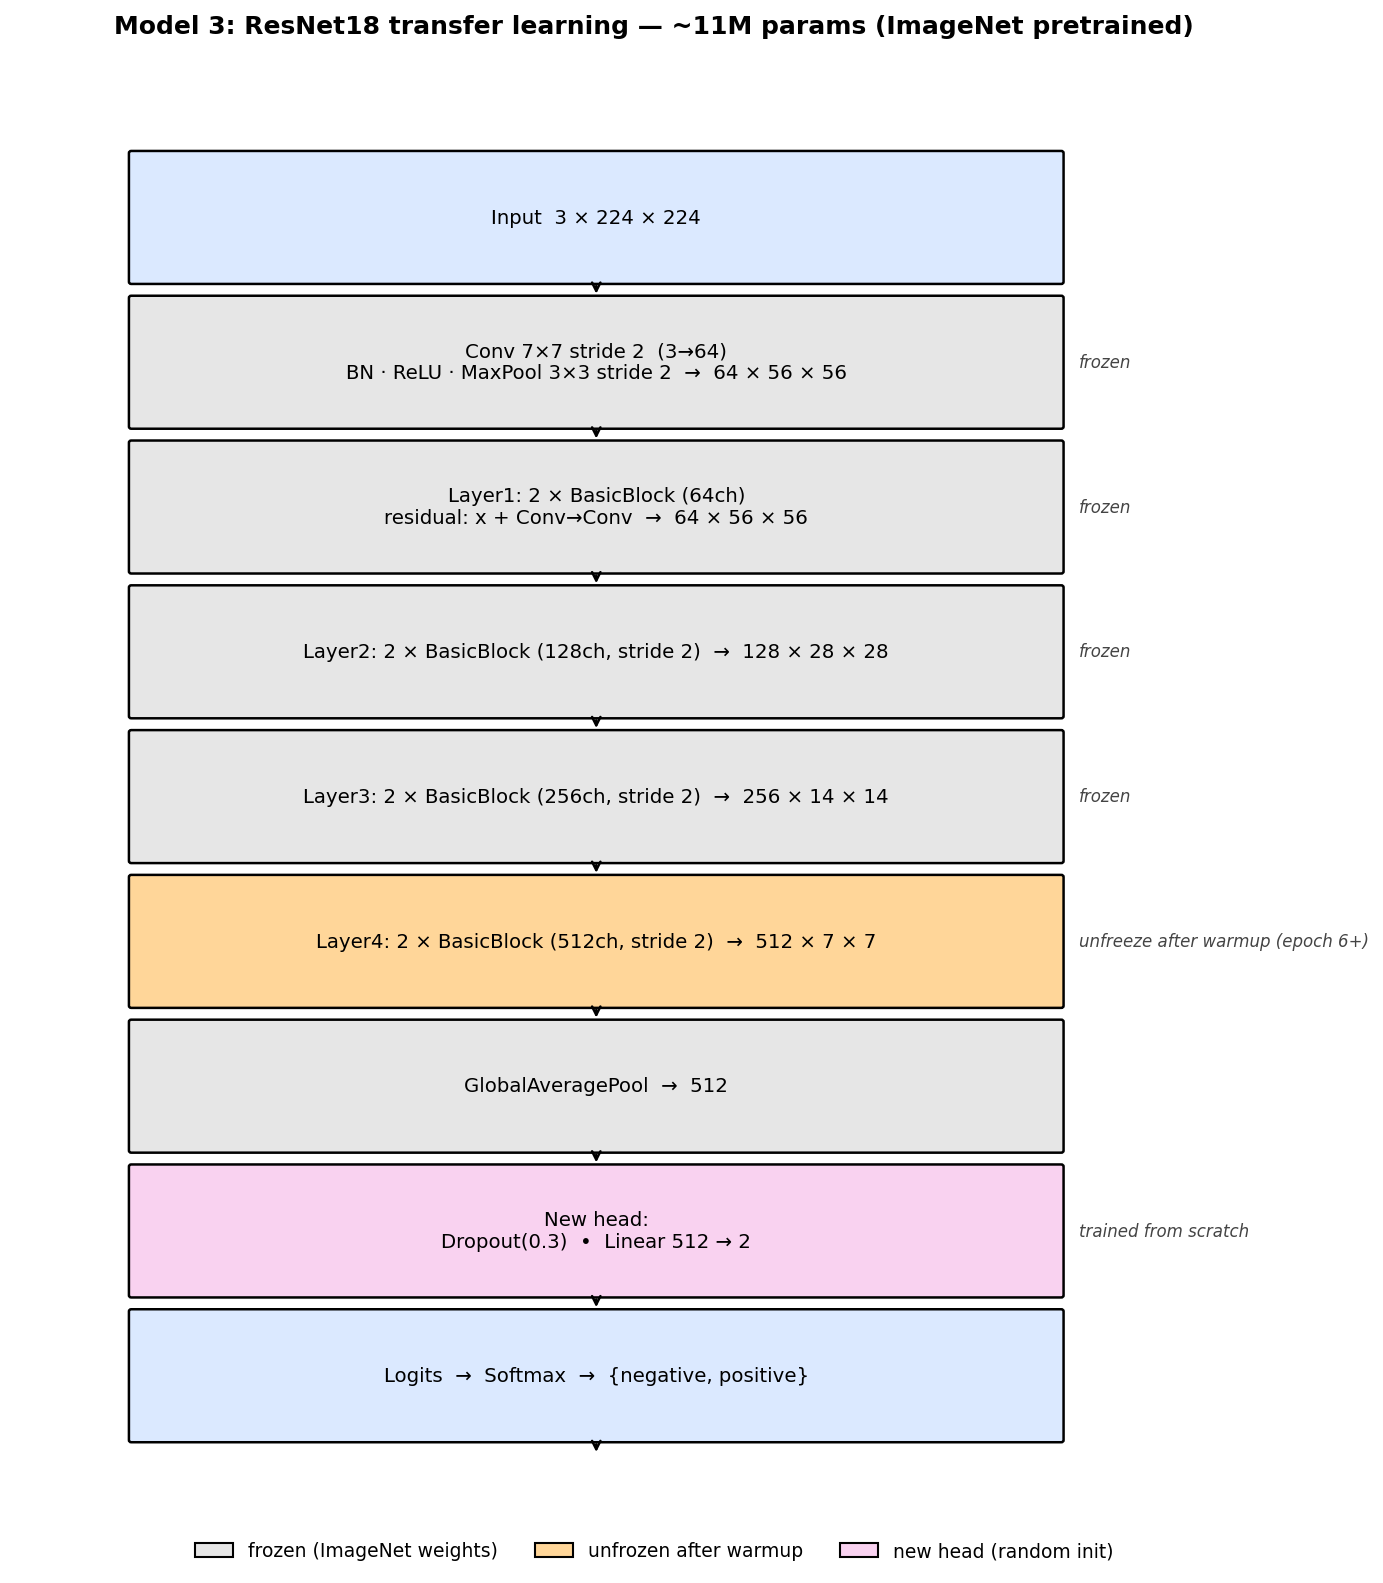
\includegraphics[width=\linewidth]{arch_resnet.png}
    \caption{Two-phase transfer-learning scheme, illustrated with ResNet18. The ImageNet-pretrained backbone is frozen during a short head-only warm-up, its deepest stage is then unfrozen for fine-tuning, and a new classifier head is trained from scratch. ResNet50, EfficientNet-B0, and ConvNeXt-Tiny follow the same procedure at a $224\times224$ input resolution.}
    \label{fig:arch_resnet}
\end{figure}

\section{Experimental Setup}
\subsection{Split Protocol}
The data split followed a four-way stratified protocol over vehicle type and class, producing 70/15/15 training, validation, and test partitions. This ensures that bus-safe, bus-unsafe, leguna-safe, and leguna-unsafe samples occur in both validation and test sets. Augmentation was applied only after splitting and only to training originals. Thresholds were tuned on validation predictions, while the 79-image test set remained untouched until final evaluation. The ensemble members (ResNet50 and ConvNeXt-Tiny) and all decision thresholds were fixed on the validation set before any test-set evaluation, so the test set was used exactly once and never for model selection, ensemble construction, or threshold tuning. The full nine-model test table is reported for transparency and did not drive the choice of the deployed model.

\subsection{Model Configuration}
The experiments were implemented in Python using scikit-learn for the classical pipelines \cite{pedregosa2011sklearn}, PyTorch for the neural model \cite{paszke2019pytorch}, and scikit-image for image processing \cite{vanderwalt2014skimage}. A fixed random seed of 42 was used for reproducibility. Model and preprocessing settings are consolidated in Table~\ref{tab:model_config}.

\begin{table*}[!t]
\centering
\caption{Model Configuration}
\label{tab:model_config}
\footnotesize
\begin{tabularx}{\textwidth}{l l X}
\toprule
\textbf{Model / Stage} & \textbf{Input Representation} & \textbf{Key Configuration} \\
\midrule
Image standardization & Source images & Orientation correction, RGB conversion, shorter side 512 px, center crop to $512\times512$, PNG output. \\
HOG feature extraction & Grayscale $128\times128$ & 9 orientation bins, $16\times16$ pixel cells, $2\times2$ cell blocks, L2-Hys normalization, 1764-d feature vector. \\
Logistic Regression & HOG features & StandardScaler and PCA (95\% variance retained) on training data, then Logistic Regression (\texttt{lbfgs}, balanced class weights). \\
Gaussian Naive Bayes & HOG features & StandardScaler and PCA (95\% variance retained) on training data, then Gaussian Naive Bayes. \\
SVM with RBF kernel & HOG features & StandardScaler and PCA (95\% variance retained) on training data; RBF-kernel SVM with penalty $C$, kernel width $\gamma$, and kernel selected by 5-fold \texttt{GridSearchCV} (balanced class weights, probability estimates enabled). \\
CNN (from scratch) & RGB $128\times128$ & Four convolutional blocks (32/64/128/256 channels) with batch normalization and ReLU, global average pooling, dropout, and a two-layer linear head; about 1.2M parameters. \\
ResNet18 & RGB $224\times224$ & ImageNet-pretrained residual network, two-phase fine-tuning. \\
EfficientNet-B0 & RGB $224\times224$ & ImageNet-pretrained compound-scaled network, two-phase fine-tuning. \\
ResNet50 & RGB $224\times224$ & Deeper ImageNet-pretrained residual network, two-phase fine-tuning, horizontal-flip TTA. \\
ConvNeXt-Tiny & RGB $224\times224$ & ImageNet-pretrained modern convolutional network, two-phase fine-tuning, horizontal-flip TTA. \\
Ensemble & RGB $224\times224$ & Probability-level average of ResNet50 and ConvNeXt-Tiny, with balanced, high-recall, and max-recall thresholds tuned on validation. \\
Deep-model training & RGB tensors & AdamW optimizer, cosine-annealing learning rate, two-phase schedule (head-only warm-up for about 5 epochs, then full-network fine-tuning), batch size 24--32, 45--70 epochs, label smoothing 0.05, dropout 0.4, weighted sampling, and class-weighted or focal loss for imbalance. \\
Evaluation protocol & Train/validation/test & Four-way stratified 70/15/15 split; 365 training originals expanded to 2,730 train images, with 79 unaugmented validation and 79 untouched test images. \\
\bottomrule
\end{tabularx}
\end{table*}

For HOG-based models, preprocessing and dimensionality-reduction steps were fitted on the training data and then applied to validation and test data. Deep models used normalized RGB image tensors rather than HOG descriptors.

For neural-model inference, the output logits $\mathbf{z} = (z_0, z_1) \in \mathbb{R}^{2}$ are mapped to class probabilities by the softmax function,
\begin{equation}
p_k = \frac{\exp(z_k)}{\sum_{j=0}^{1} \exp(z_j)}, \qquad k \in \{0, 1\},
\end{equation}
so that $p_1$ is the estimated probability of the unsafe class.
Neural models were trained with the AdamW optimizer, a decoupled weight-decay variant of Adam \cite{kingma2015adam}, under a cosine-annealing learning-rate schedule; the complete training configuration is listed in Table~\ref{tab:model_config}.

\subsection{Evaluation Metrics}
Evaluation used accuracy, balanced accuracy, precision, recall, specificity, the $F_1$-score, the Matthews correlation coefficient (MCC), ROC-AUC, and PR-AUC. Because the classes are close to balanced, both ROC-AUC and PR-AUC are reported, and per-class recall is emphasized for the safety-critical unsafe class. Let $TP$, $TN$, $FP$, and $FN$ denote the numbers of true positives, true negatives, false positives, and false negatives, with the positive class corresponding to unsafe/risky hanging travel. The threshold-dependent metrics are then defined as
\begin{align}
\mathrm{Accuracy} &= \frac{TP + TN}{TP + TN + FP + FN}, \label{eq:acc}\\[2pt]
\mathrm{Precision} &= \frac{TP}{TP + FP}, \qquad
\mathrm{Recall} = \frac{TP}{TP + FN}, \label{eq:prrec}\\[2pt]
\mathrm{Specificity} &= \frac{TN}{TN + FP}, \label{eq:spec}\\[2pt]
F_1 &= \frac{2\,\mathrm{Precision} \cdot \mathrm{Recall}}{\mathrm{Precision} + \mathrm{Recall}}
= \frac{2\,TP}{2\,TP + FP + FN}. \label{eq:f1}
\end{align}
Recall (equivalently, sensitivity or the true positive rate) quantifies unsafe-class coverage, whereas specificity (the true negative rate) quantifies safe-class coverage. Because a single decision threshold can favor one class, balanced accuracy reports the unweighted mean of the two per-class recalls and is therefore insensitive to class prevalence,
\begin{equation}
\begin{split}
\mathrm{Balanced\ Accuracy}
&= \frac{\mathrm{Recall} + \mathrm{Specificity}}{2} \\
&= \frac{1}{2}\!\left(\frac{TP}{TP + FN} + \frac{TN}{TN + FP}\right). \label{eq:bacc}
\end{split}
\end{equation}
The Matthews correlation coefficient (MCC) is the Pearson correlation coefficient between the predicted and true binary labels. It combines all four confusion-matrix cells and attains a high value only when the classifier performs well on both classes simultaneously, which makes it a reliable single-number summary under class imbalance \cite{chicco2020mcc}:
\begin{equation}
\mathrm{MCC} = \frac{TP \cdot TN - FP \cdot FN}
{\sqrt{(TP{+}FP)(TP{+}FN)(TN{+}FP)(TN{+}FN)}}. \label{eq:mcc}
\end{equation}
The coefficient lies in $[-1, +1]$, where $+1$ indicates perfect prediction, $0$ chance-level prediction, and $-1$ total disagreement; when any factor in the denominator is zero, it is taken as $0$ by convention. Two threshold-independent metrics summarize ranking quality across all decision thresholds. ROC-AUC is the area under the receiver operating characteristic curve, which plots the true positive rate against the false positive rate, and equals the probability that a randomly chosen unsafe image is scored above a randomly chosen safe one. PR-AUC (average precision) is the area under the precision--recall curve,
\begin{equation}
\mathrm{AP} = \sum_{n} \left(R_n - R_{n-1}\right) P_n, \label{eq:ap}
\end{equation}
where $P_n$ and $R_n$ are the precision and recall at the $n$-th threshold; its no-skill baseline equals the unsafe-class prevalence, which makes it informative for the safety-critical positive class. Because missed unsafe cases have direct safety implications, unsafe-class recall is emphasized alongside overall accuracy, MCC, and AUC. Given the small test set, uncertainty is reported as 95\% Wilson score intervals, and pairwise differences between the strongest models are assessed with McNemar's exact test.


\section{Results}
\subsection{Quantitative Comparison}
Table~\ref{tab:test_results} reports balanced operating-point performance on the untouched 79-image test set. The ResNet50--ConvNeXt ensemble reaches 0.861 accuracy, 0.947 unsafe recall, and 0.970 ROC-AUC. ResNet50 attains the highest single-model accuracy (0.924) and MCC (0.848), while EfficientNet-B0 attains the highest unsafe recall (0.974) and ROC-AUC (0.979). All nine models are compared in Fig.~\ref{fig:paper_model_comparison}.

\begin{table*}[!t]
\centering
\caption{Held-out Test Performance for All Reported Models}
\label{tab:test_results}
\footnotesize
\setlength{\tabcolsep}{3pt}
\resizebox{\textwidth}{!}{%
\begin{tabular}{lccccccccc}
\toprule
\textbf{Model} & \textbf{Acc.} & \textbf{Bal. Acc.} & \textbf{Unsafe R} & \textbf{Unsafe P} & \textbf{Spec.} & \textbf{$F_1$} & \textbf{AUC} & \textbf{PR-AUC} & \textbf{MCC} \\
\midrule
Ensemble & 0.861 & 0.864 & 0.947 & 0.800 & 0.780 & 0.867 & 0.970 & 0.978 & 0.734 \\
ResNet50 & \textbf{0.924} & \textbf{0.924} & 0.921 & \textbf{0.921} & \textbf{0.927} & \textbf{0.921} & 0.967 & 0.975 & \textbf{0.848} \\
ConvNeXt-Tiny & 0.835 & 0.840 & 0.947 & 0.766 & 0.732 & 0.847 & 0.972 & 0.979 & 0.691 \\
EfficientNet-B0 & 0.835 & 0.841 & \textbf{0.974} & 0.755 & 0.707 & 0.851 & \textbf{0.979} & \textbf{0.980} & 0.701 \\
ResNet18 & 0.911 & 0.912 & 0.921 & 0.897 & 0.902 & 0.909 & 0.971 & 0.976 & 0.823 \\
CNN & 0.861 & 0.861 & 0.868 & 0.846 & 0.854 & 0.857 & 0.929 & 0.896 & 0.722 \\
SVM (RBF) & 0.873 & 0.874 & 0.895 & 0.850 & 0.854 & 0.872 & 0.952 & 0.958 & 0.748 \\
Logistic Regression & 0.810 & 0.810 & 0.816 & 0.795 & 0.805 & 0.805 & 0.887 & 0.900 & 0.620 \\
Naive Bayes & 0.734 & 0.734 & 0.737 & 0.718 & 0.732 & 0.727 & 0.866 & 0.884 & 0.468 \\
\bottomrule
\end{tabular}
}
\end{table*}

\begin{figure*}[!t]
    \centering
    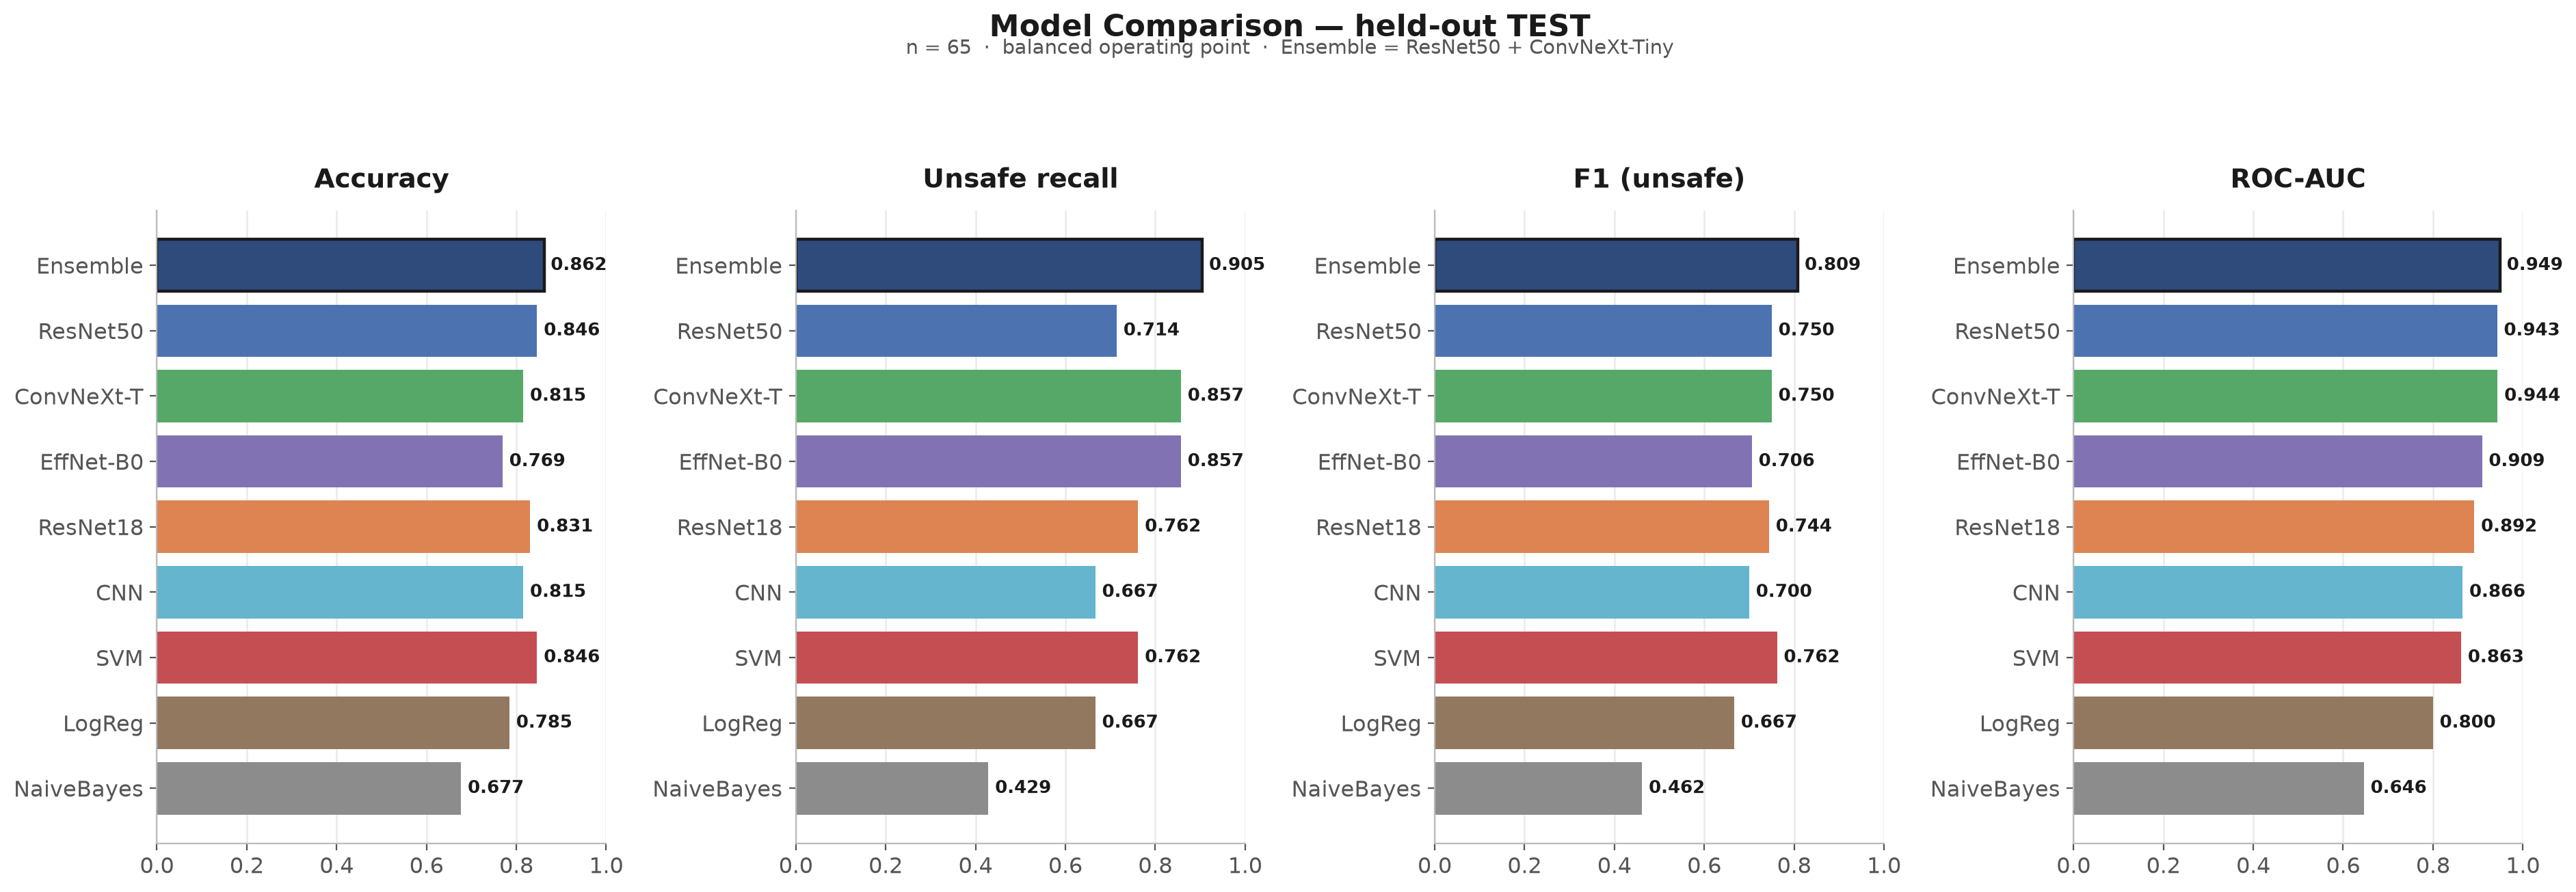
\includegraphics[width=\textwidth]{figures/fig02_model_comparison.png}
    \caption{Held-out test comparison of accuracy, unsafe recall, unsafe $F_1$, and ROC-AUC across all nine reported models.}
    \label{fig:paper_model_comparison}
\end{figure*}

\subsection{ROC and AUC Analysis}
AUC values are reported in Table~\ref{tab:test_results}. Figure~\ref{fig:paper_roc_test} shows held-out ROC curves for all reported models, and Fig.~\ref{fig:paper_pr_curves} shows the corresponding precision--recall curves.

\begin{figure*}[t]
    \centering
    \subfloat[ROC curves.\label{fig:paper_roc_test}]{%
        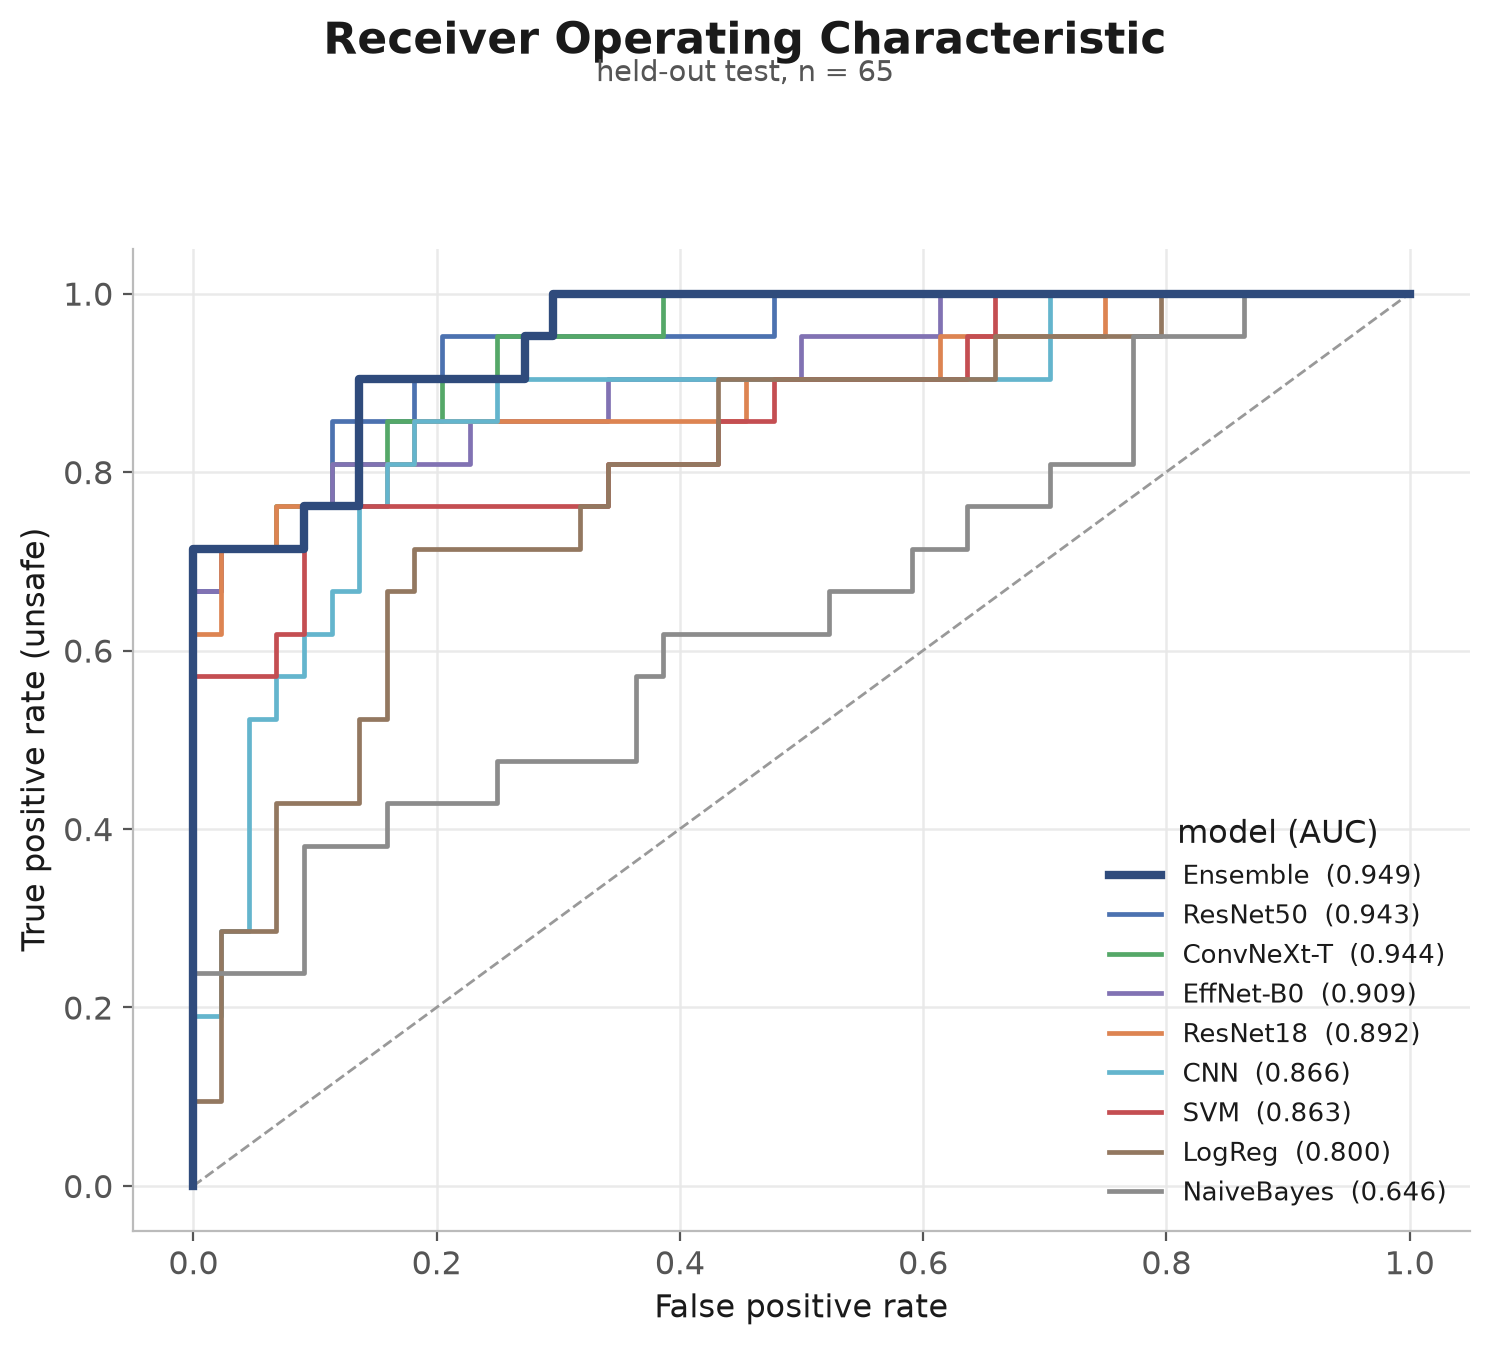
\includegraphics[width=0.49\textwidth]{figures/fig03_roc_test.png}}
    \hfill
    \subfloat[Precision--recall curves.\label{fig:paper_pr_curves}]{%
        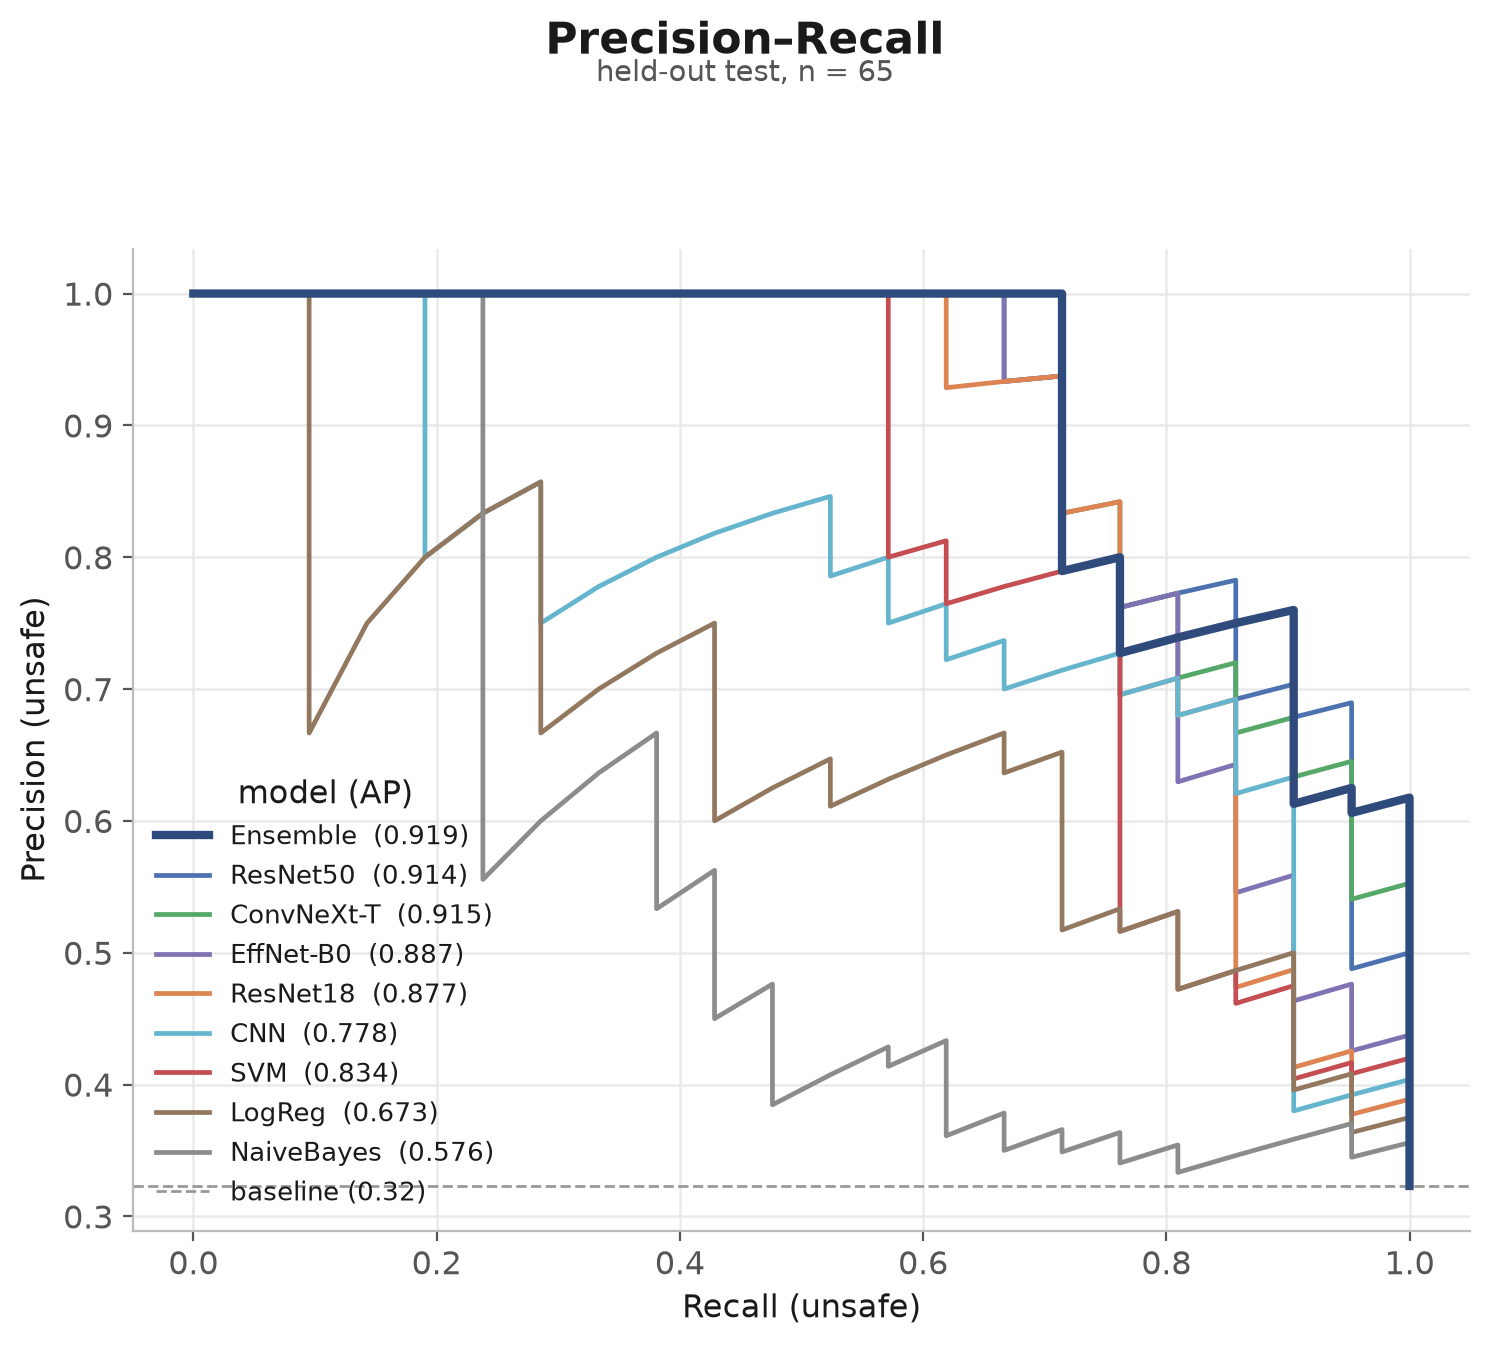
\includegraphics[width=0.49\textwidth]{figures/fig04_pr_curves.png}}
    \caption{Receiver operating characteristic and precision--recall curves for all nine models on the held-out test set.}
    \label{fig:classwise_curve_analysis}
\end{figure*}

\subsection{Error Analysis}
False negatives are the most safety-critical error type because they correspond to unsafe/risky hanging-travel cases predicted as safe/normal. At the balanced operating point, the ensemble detects 94.7\% of unsafe test images, missing only 2 of 38 hangers. Because the retrained dataset is close to balanced, the tuned balanced, high-recall, and max-recall thresholds fall within 0.006 of one another, so all three settle at the same operating point of 86.1\% accuracy and 94.7\% unsafe recall. The earlier regime, in which perfect recall could only be bought at low accuracy, no longer appears: the additional unsafe training data lets the ensemble reach high recall without sacrificing accuracy. Table~\ref{tab:operating_modes} lists the three modes, and Fig.~\ref{fig:operating_analysis} shows the threshold trade-off.

\begin{table}[t]
\centering
\caption{Selectable operating points for the deployed ensemble. On the near-balanced retrained data the three tuned thresholds nearly coincide, so the modes report the same test operating point.}
\label{tab:operating_modes}
\footnotesize
\setlength{\tabcolsep}{4pt}
\resizebox{\linewidth}{!}{%
\begin{tabular}{lccccc}
\toprule
\textbf{Mode} & \textbf{Threshold} & \textbf{Test Acc.} & \textbf{Unsafe R} & \textbf{Unsafe P} & \textbf{Spec.} \\
\midrule
Balanced & 0.170 & 0.861 & 0.947 & 0.800 & 0.780 \\
High recall & 0.175 & 0.861 & 0.947 & 0.800 & 0.780 \\
Max recall & 0.175 & 0.861 & 0.947 & 0.800 & 0.780 \\
\bottomrule
\end{tabular}
}
\end{table}

\begin{figure}[!t]
    \centering
    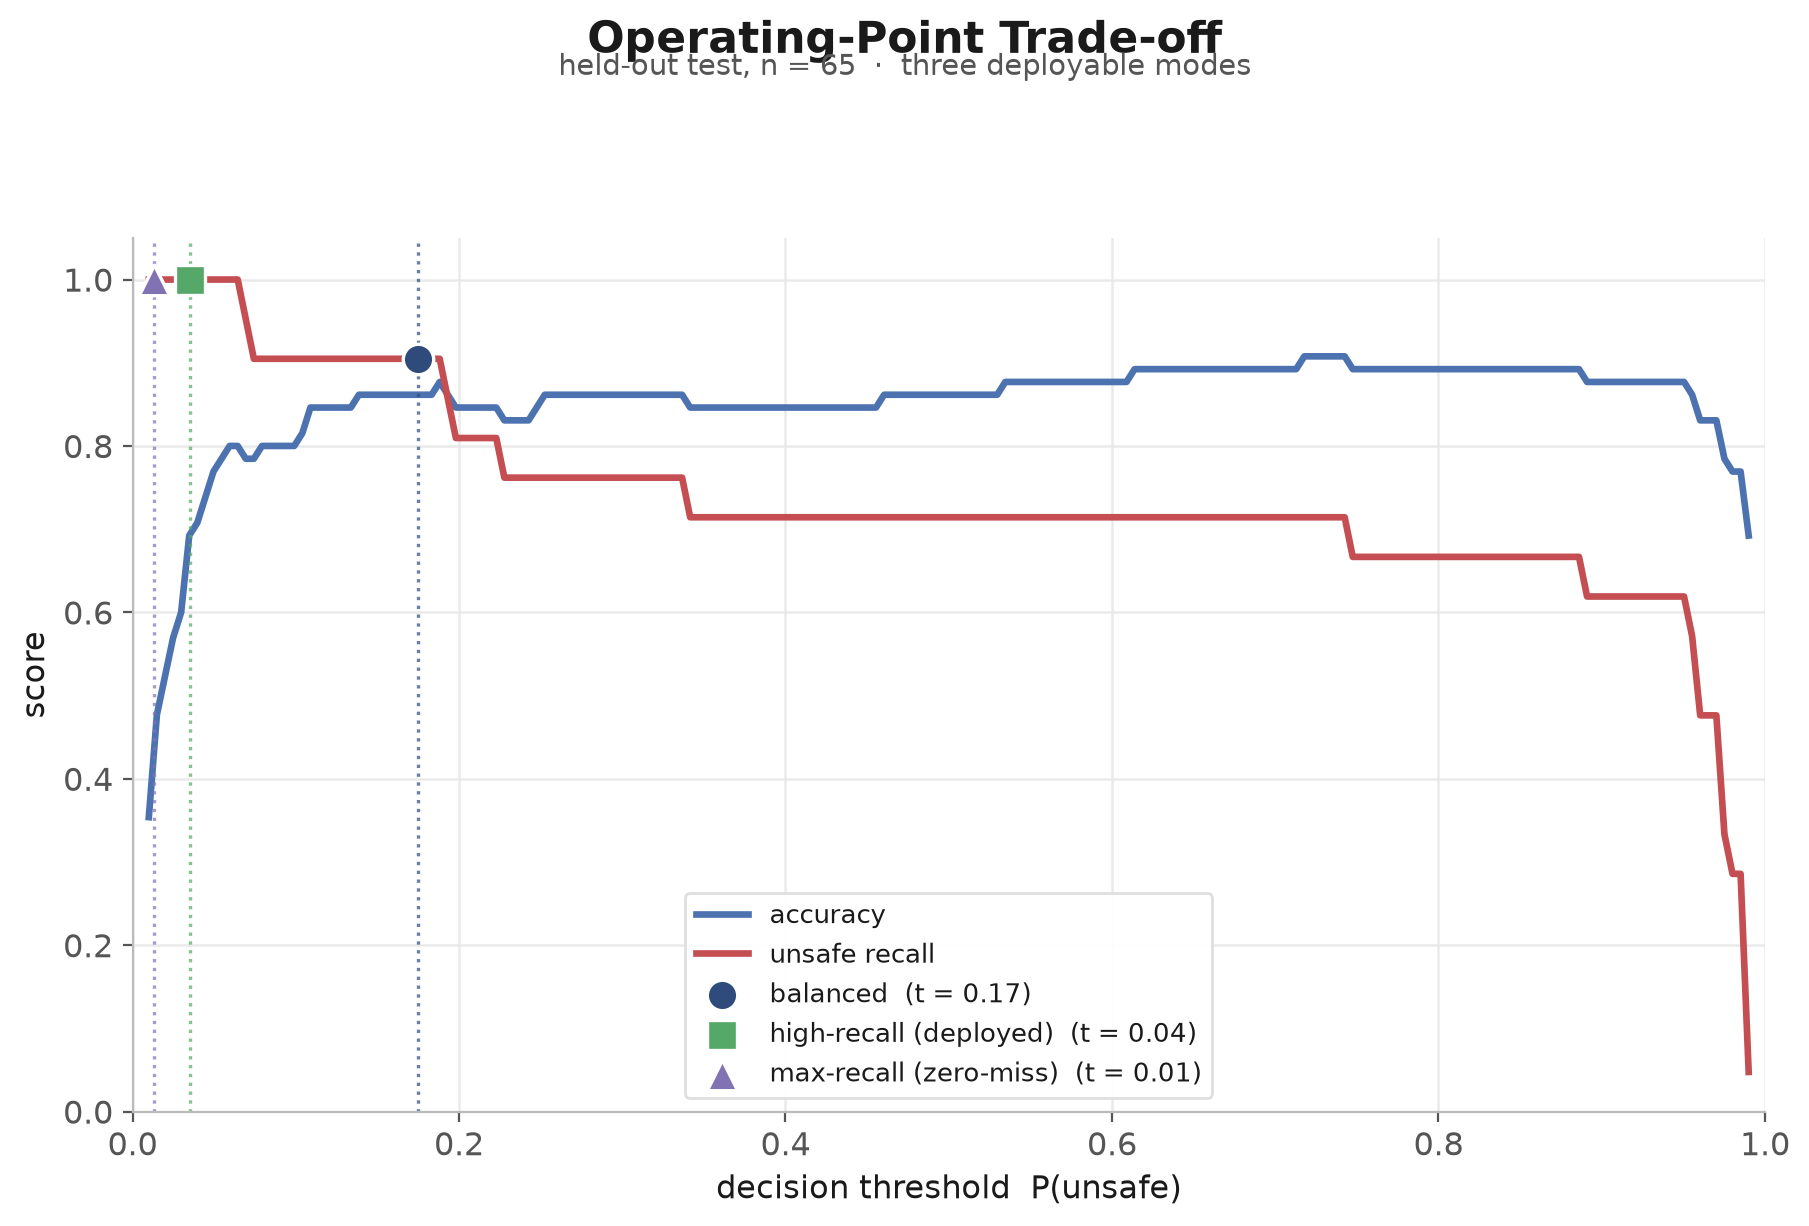
\includegraphics[width=\linewidth]{figures/fig06_tradeoff.png}
    \caption{Ensemble threshold selection on the held-out test set: accuracy and unsafe recall against the decision threshold, with the balanced, high-recall, and max-recall operating points marked. Because the retrained dataset is near-balanced, the three points nearly coincide.}
    \label{fig:operating_analysis}
\end{figure}

\section{Discussion}
\subsection{Interpretation of Results}
The retrained ensemble provides a strong, recall-oriented balanced operating point, reaching 86.1\% test accuracy, 94.7\% unsafe recall, 0.867 unsafe $F_1$, 0.970 ROC-AUC, and 0.978 PR-AUC. The additional unsafe training data raises AUC beyond the previous 0.949 result and substantially improves balanced unsafe recall.

Among individual deep models, ResNet50 leads on accuracy (92.4\%) with balanced 92.1\% unsafe precision and recall, while EfficientNet-B0 reaches the highest unsafe recall (97.4\%) and the top ROC-AUC (0.979). Among classical models, SVM remains the strongest HOG baseline, reaching 87.3\% accuracy, 89.5\% unsafe recall, and 0.952 AUC.

We deploy the ResNet50--ConvNeXt ensemble rather than the single most accurate model because the two error types carry asymmetric cost: a false negative, a missed hanging passenger, is more consequential than a false alarm. The ensemble attains 94.7\% unsafe recall, above ResNet50's 92.1\%, and averaging two backbones yields probabilities that are more stable across the operating thresholds than any single network. EfficientNet-B0 reaches an even higher unsafe recall (97.4\%) and is a strong recall-oriented alternative, but its lower balanced accuracy (83.5\%) produces more false alarms, so the ensemble was retained for its better accuracy--recall balance.

Gaussian Naive Bayes underperforms because its conditional-independence assumption is poorly matched to HOG descriptors. Neighboring gradient bins and block-normalized features are correlated by construction, so treating them as independent weakens the model's ability to distinguish visually similar safe/normal and unsafe/risky scenes.

The train-to-test gaps in Table~\ref{tab:generalization} range from 6.7 to 16.5 percentage points. Logistic Regression has the smallest gap, while ConvNeXt-Tiny has the largest. These gaps are markedly smaller than in the previous run, which indicates that the expanded set of unique originals reduces overfitting, even though it does not remove it entirely. Figure~\ref{fig:generalization_analysis} visualizes the per-model train, validation, and test error and the train-to-test gap.

For this application, false negatives are more consequential than ordinary classification errors because they correspond to missed risky travel conditions. Precision and overall accuracy remain relevant for reducing false alarms, but a safety-oriented monitoring system should prioritize reducing missed unsafe cases while maintaining acceptable discrimination across normal and risky scenes.

\subsection{Limitations}
The main limitation of this study is the limited number of unique source images. The updated dataset contains 523 labeled originals with 251 unsafe cases, which is still not enough to fully cover the diversity of vehicle layouts, camera viewpoints, passenger postures, weather, illumination, and traffic environments encountered in deployment. With only 79 test images, individual metrics carry wide uncertainty: a 95\% Wilson score interval on the ensemble's 86.1\% accuracy spans $[76.8, 92.0]\%$. A McNemar exact test finds no significant difference among the strongest models (for example, ResNet50 versus the ensemble gives $p = 0.125$ and ResNet50 versus ResNet18 gives $p = 1.0$), so these models are statistically indistinguishable on this test set, and the per-metric maxima in Table~\ref{tab:test_results} should be read as descriptive rather than as proof of a single definitively best model. Because nine models are compared on one split, the top scores are also subject to selection (``winner's-curse'') optimism, and the reported interval captures only test-set sampling noise, not train/validation-split or random-seed variability. Cross-validated or repeated-seed evaluation would tighten these estimates and is left to future work.

The neural models also depend on training-time augmentation to increase effective sample diversity. Augmentation makes the models less sensitive to controlled transformations, but it does not replace additional real images containing natural occlusion, motion blur, dense crowding, and non-standard bus or leguna structures. These factors can make unsafe/risky positive cases difficult to distinguish from visually cluttered safe/normal scenes.

The current system is limited to image-level binary classification. It does not localize hanging passengers, estimate crowd density, track passengers across frames, or evaluate performance on large-scale real-time video streams. Roadside transport images may also include identifiable people, license plates, and location cues, so deployment would require anonymization and data-governance safeguards. The method should therefore be interpreted as a baseline for visual safety classification rather than an operational monitoring system.

\begin{table}[!t]
\centering
\caption{Train, Validation, and Test Generalization}
\label{tab:generalization}
\footnotesize
\setlength{\tabcolsep}{2pt}
\resizebox{\linewidth}{!}{%
\begin{tabular}{lccccccc}
\toprule
\textbf{Model} & \textbf{Train Acc.} & \textbf{Train Err.} & \textbf{Val Acc.} & \textbf{Val Err.} & \textbf{Test Acc.} & \textbf{Test Err.} & \textbf{Test R} \\
\midrule
Ensemble & 0.999 & 0.001 & 0.962 & 0.038 & 0.861 & 0.139 & 0.947 \\
ResNet50 & 0.997 & 0.003 & 0.962 & 0.038 & 0.924 & 0.076 & 0.921 \\
ConvNeXt-Tiny & 1.000 & 0.000 & 0.962 & 0.038 & 0.835 & 0.165 & 0.947 \\
EfficientNet-B0 & 0.989 & 0.011 & 0.937 & 0.063 & 0.835 & 0.165 & 0.974 \\
ResNet18 & 0.996 & 0.004 & 0.949 & 0.051 & 0.911 & 0.089 & 0.921 \\
CNN & 0.962 & 0.038 & 0.937 & 0.063 & 0.861 & 0.139 & 0.868 \\
SVM (RBF) & 0.999 & 0.001 & 0.861 & 0.139 & 0.873 & 0.127 & 0.895 \\
Logistic Regression & 0.877 & 0.123 & 0.772 & 0.228 & 0.810 & 0.190 & 0.816 \\
Naive Bayes & 0.832 & 0.168 & 0.810 & 0.190 & 0.734 & 0.266 & 0.737 \\
\bottomrule
\end{tabular}
}
\end{table}

\begin{figure}[!t]
    \centering
    \subfloat[Train, validation, and test error.\label{fig:generalization_error}]{%
        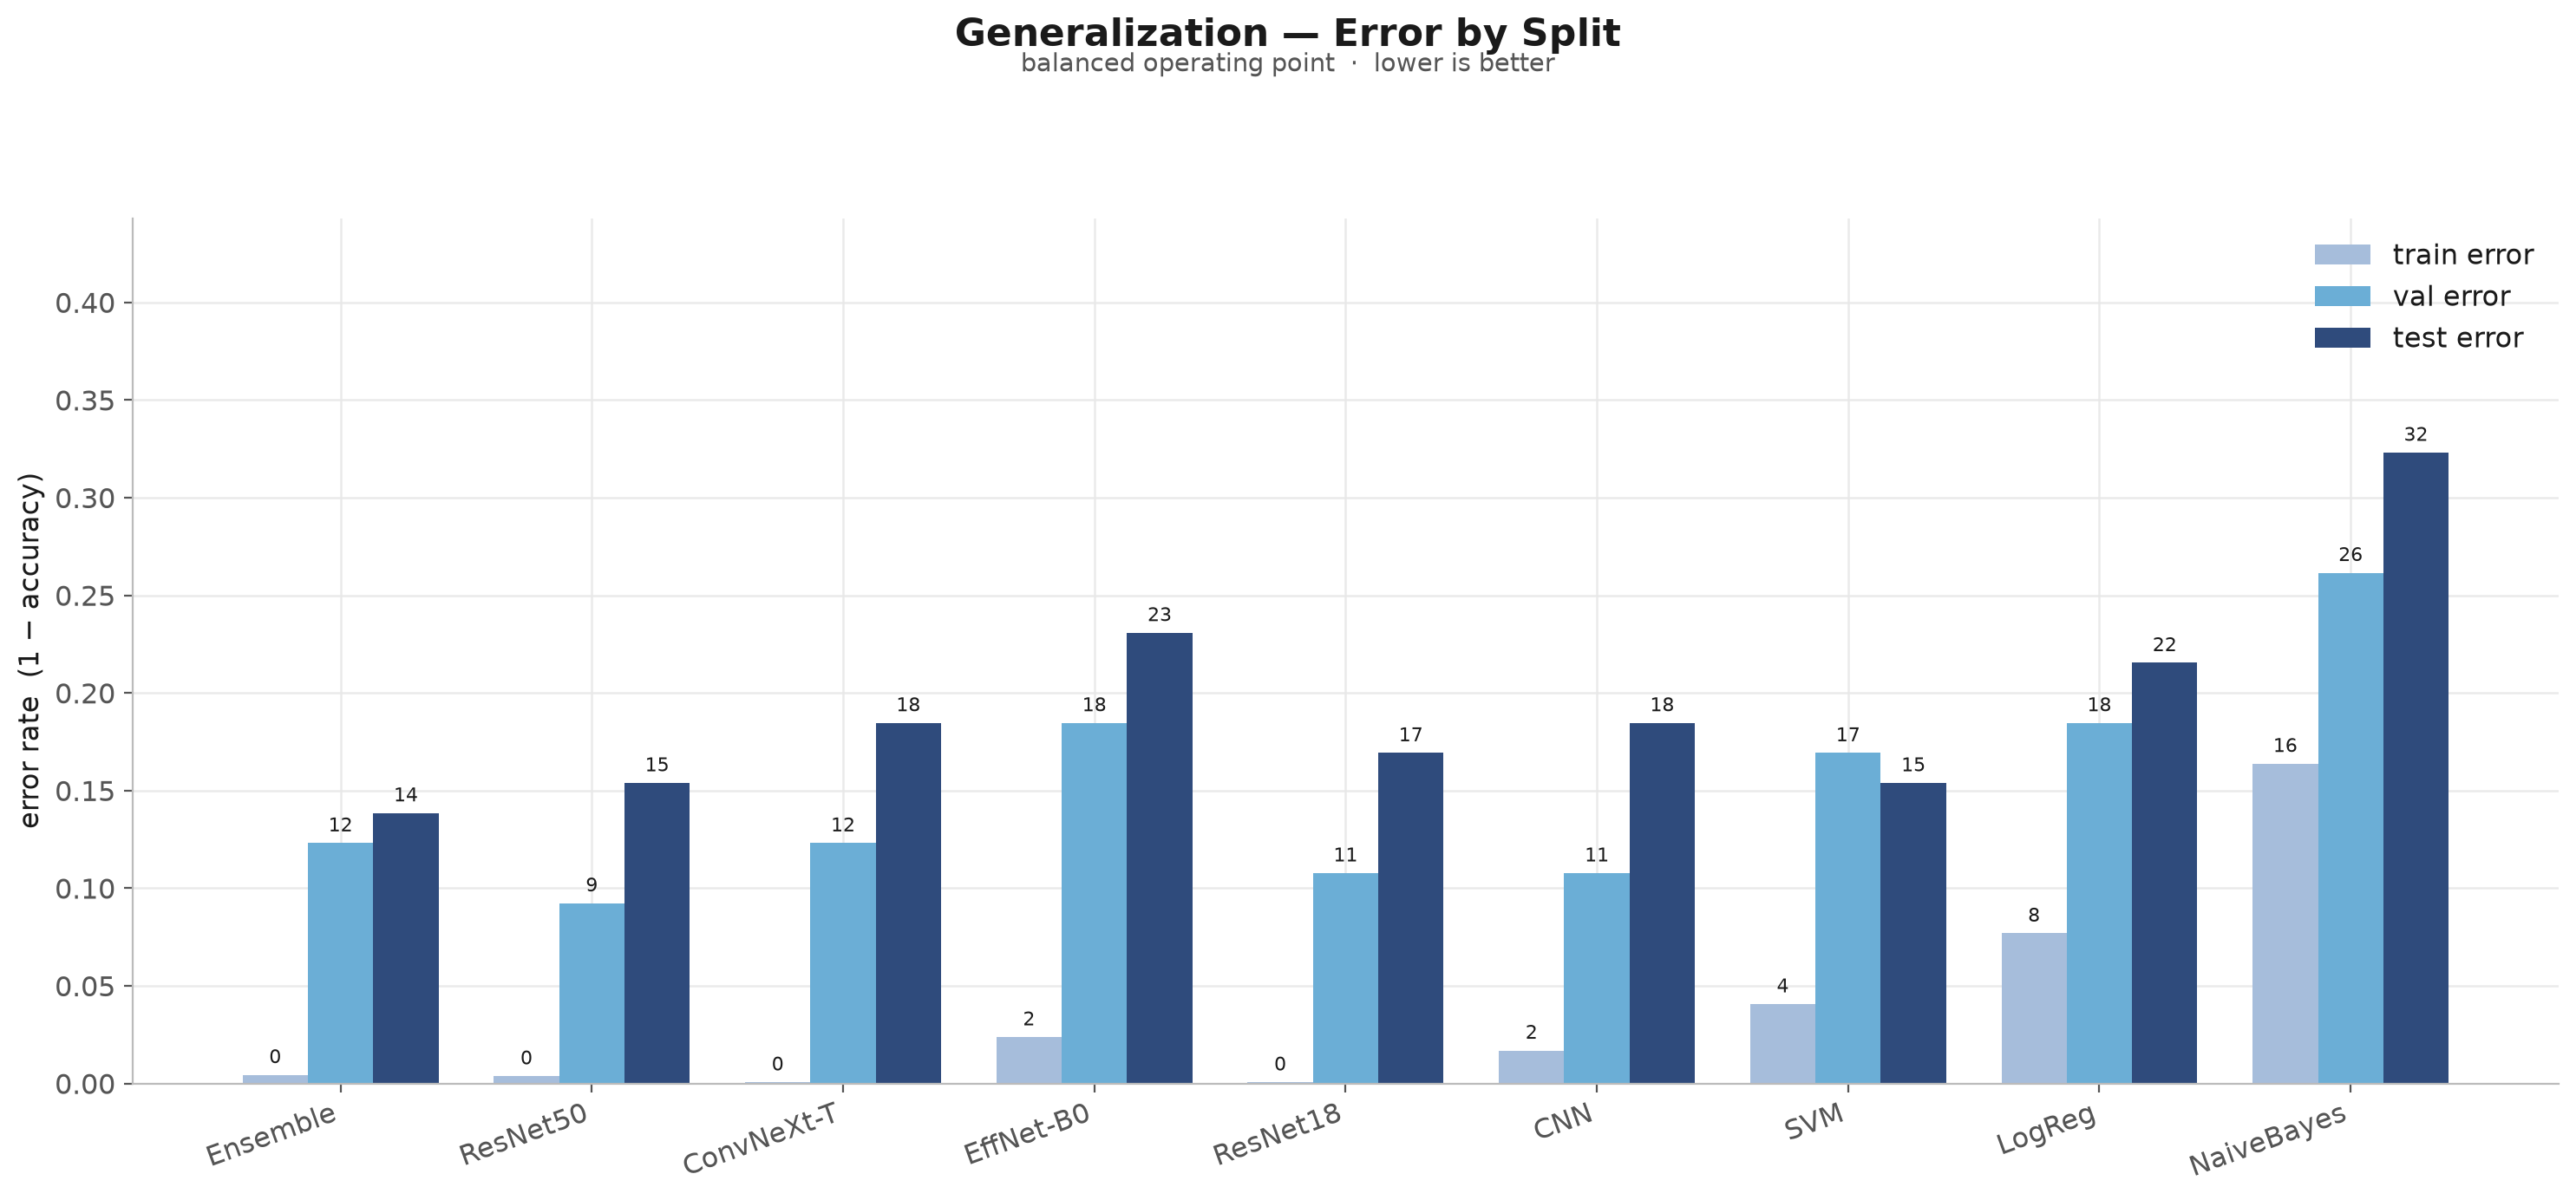
\includegraphics[width=\linewidth]{figures/fig07_train_val_test_error.png}}
    \par\smallskip
    \subfloat[Train-to-test generalization gap.\label{fig:generalization_gap}]{%
        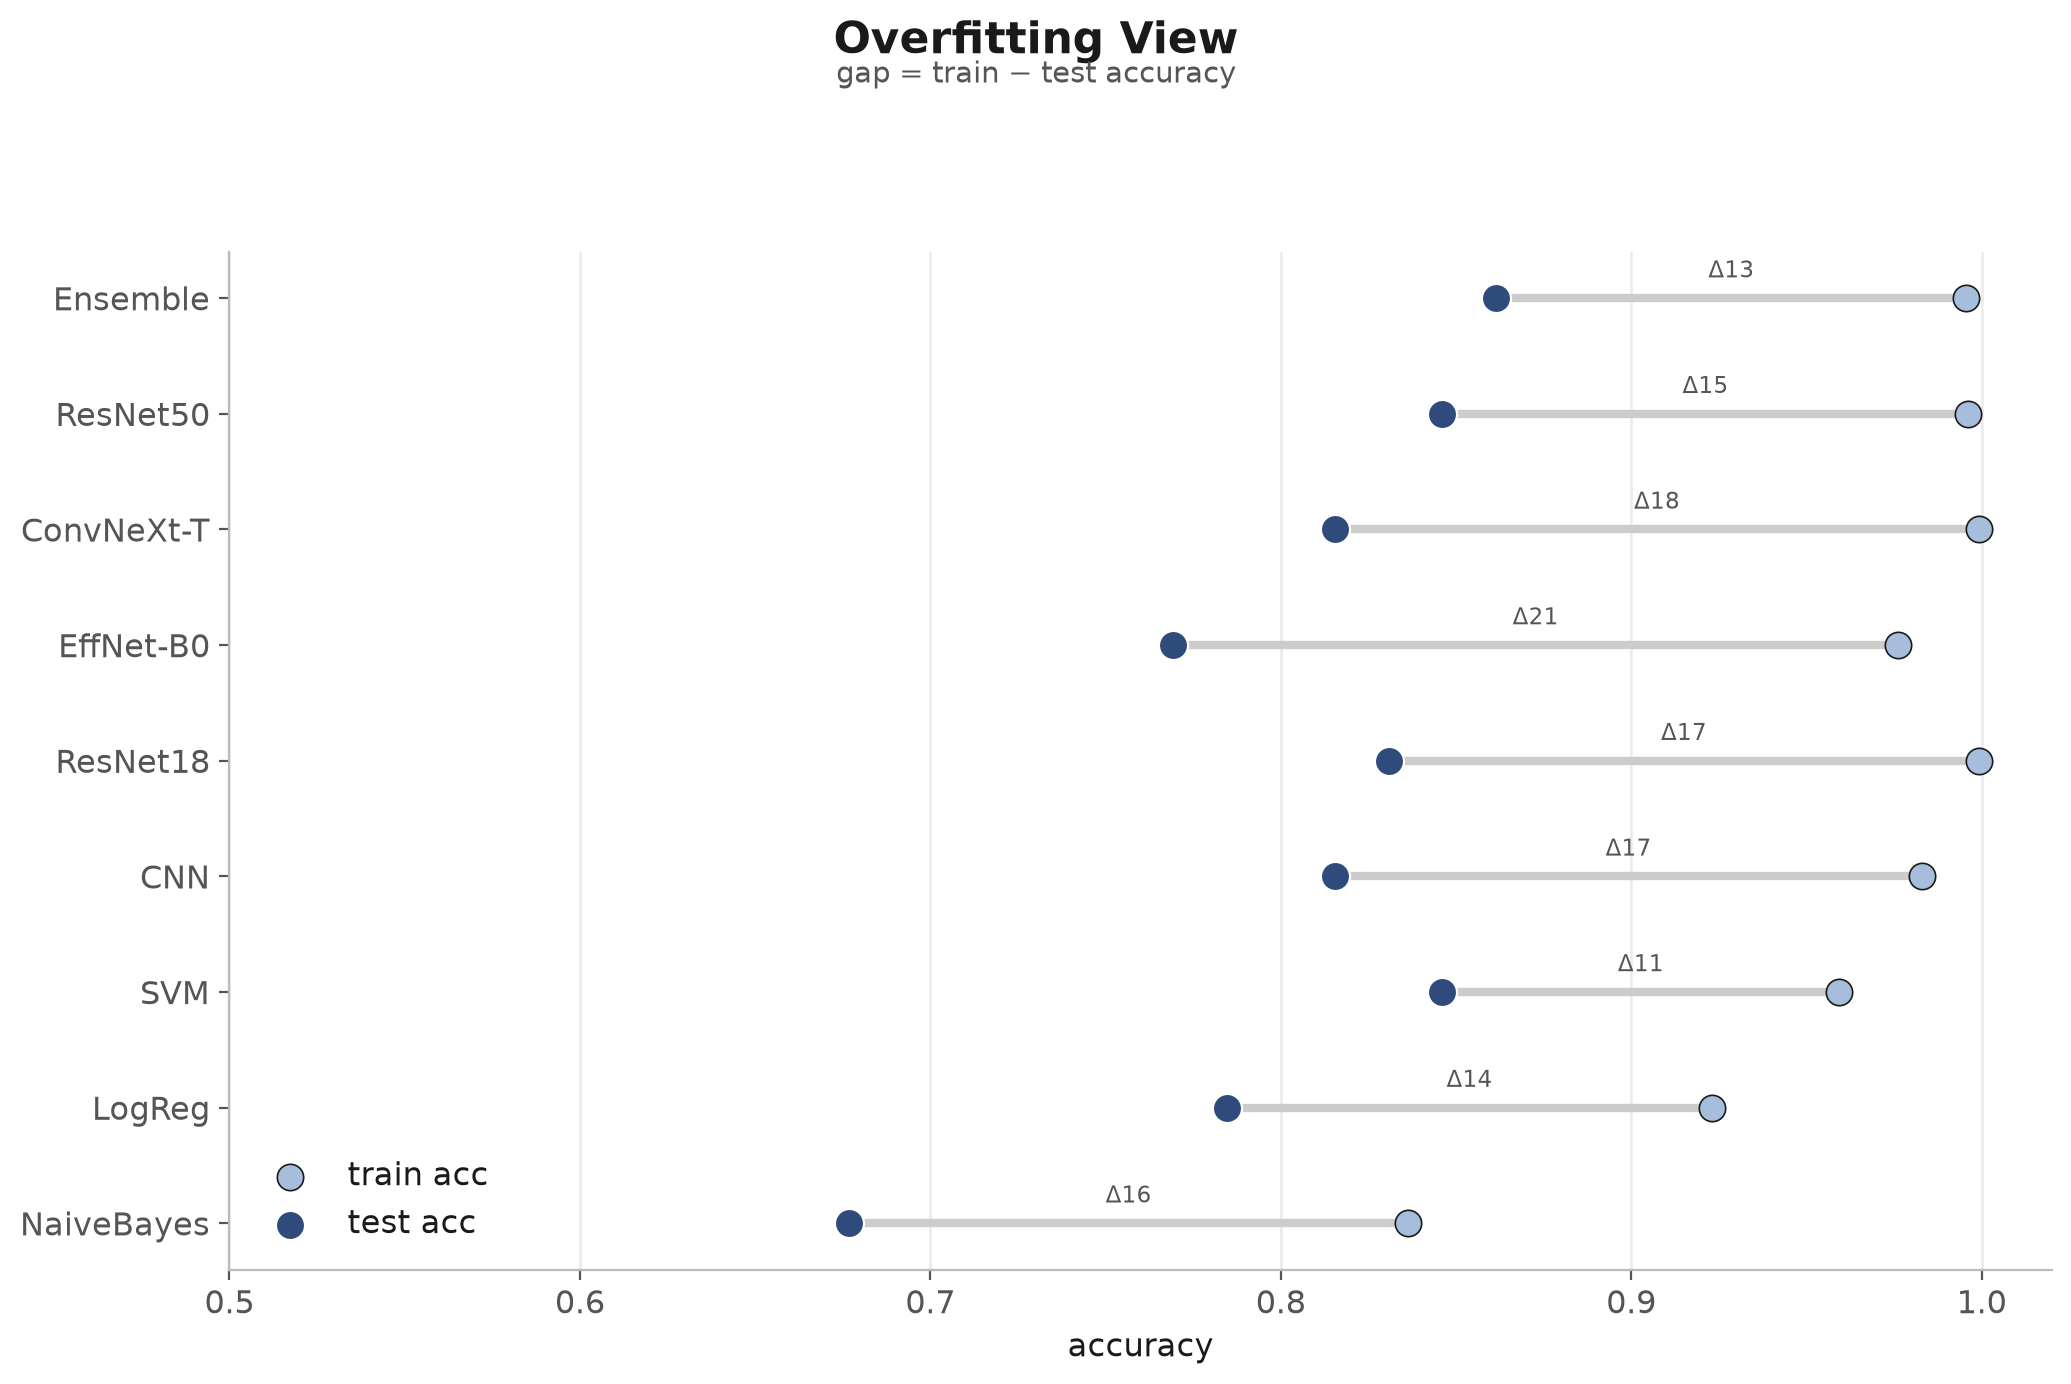
\includegraphics[width=\linewidth]{figures/fig08_generalization_gap.png}}
    \caption{Generalization behavior of all nine models after retraining.}
    \label{fig:generalization_analysis}
\end{figure}

\FloatBarrier
\section{Conclusion and Future Work}
This paper presented a computer-vision and machine-learning pipeline for detecting unsafe hanging travel in Dhaka public transport. The task was formulated as binary image classification over safe/normal and unsafe/risky passenger conditions. A localized bus and leguna dataset was prepared through cleaning, annotation, preprocessing, and augmentation, with HOG features used for classical models and RGB inputs used for CNN-based classification.

The updated result set compares Logistic Regression, Gaussian Naive Bayes, SVM with an RBF kernel, a CNN trained from scratch, ResNet18, EfficientNet-B0, ResNet50, ConvNeXt-Tiny, and a ResNet50--ConvNeXt ensemble. On the untouched test set, the deployed ensemble reaches a recall-oriented balanced result with 86.1\% accuracy, 94.7\% unsafe recall, and 0.970 ROC-AUC, while ResNet50 gives the highest single-model accuracy at 92.4\%. Because the retrained data is near-balanced, the balanced, high-recall, and max-recall thresholds coincide at the same 86.1\%-accuracy and 94.7\%-recall operating point rather than trading accuracy for a separate perfect-recall mode.

As a practical outcome of this work, we developed an online platform that allows users to classify public-transport images as safe/normal or unsafe/risky. The platform is available at \href{https://ml-predictor-app.streamlit.app/}{\texttt{ml-predictor-app.streamlit.app}}.

Future work should focus on collecting a larger localized dataset, improving recall for unsafe hanging travel, evaluating the system on real-time video streams, and designing privacy-aware deployment procedures. Detection-based models such as YOLO \cite{redmon2016yolo} should also be tested to localize hanging passengers rather than only classify whole images. License-plate recognition may be integrated only as a future extension for vehicle identification after unsafe conditions are detected.

\FloatBarrier
\begin{thebibliography}{99}

\bibitem{dilek2023cvits}
E. Dilek and M. Dener,
``Computer Vision Applications in Intelligent Transportation Systems: A Survey,''
\textit{Sensors}, vol. 23, no. 6, 2938, 2023.\\
Available: \url{https://www.mdpi.com/1424-8220/23/6/2938}

\bibitem{hsu2020passenger}
Y.-W. Hsu, T.-Y. Wang, and J.-W. Perng,
``Passenger flow counting in buses based on deep learning using surveillance video,''
\textit{Optik}, vol. 202, 163675, 2020.\\
Available: \url{https://www.sciencedirect.com/science/article/abs/pii/S0030402619315736}

\bibitem{barua2013brt}
S. Barua, M. Seraj, and D. Alam,
``Opportunities and Operational Difficulties of Introducing Bus Rapid Transit (BRT) in Dhaka,''
in \textit{Urban Public Transportation Systems 2013}, American Society of Civil Engineers, 2013, pp. 168-178.\\
Available: \url{https://doi.org/10.1061/9780784413210.016}

\bibitem{crowding2023review}
Z. Li and D. A. Hensher,
``Crowding in Public Transport: A Review of Objective and Subjective Measures,''
\textit{Journal of Public Transportation}, vol. 16, no. 2, pp. 107-134, 2013.\\
Available: \url{https://doi.org/10.5038/2375-0901.16.2.6}

\bibitem{wastupranata2024abnormal}
L. M. Wastupranata, S. G. Kong, and L. Wang,
``Deep Learning for Abnormal Human Behavior Detection in Surveillance Videos---A Survey,''
\textit{Electronics}, vol. 13, no. 13, 2579, 2024.\\
Available: \url{https://www.mdpi.com/2079-9292/13/13/2579}

\bibitem{redmon2016yolo}
J. Redmon, S. Divvala, R. Girshick, and A. Farhadi,
``You Only Look Once: Unified, Real-Time Object Detection,''
in \textit{IEEE Conference on Computer Vision and Pattern Recognition (CVPR)}, 2016, pp. 779-788.\\
Available: \url{https://arxiv.org/abs/1506.02640}

\bibitem{yolo2024boarding}
W. Xu, Y. Zhao, X. Du, H. Ji, and L. Xing,
``A Study on Bus Passenger Boarding and Alighting Detection and Recognition Based on Video Images and YOLO Algorithm,''
\textit{Sensors}, vol. 26, no. 5, 1418, 2026.\\
Available: \url{https://doi.org/10.3390/s26051418}

\bibitem{tseng2022bus}
C.-H. Tseng and H.-Y. Lin,
``A Vision-Based System for Abnormal Behavior Detection and Recognition of Bus Passengers,''
in \textit{2022 IEEE 25th International Conference on Intelligent Transportation Systems (ITSC)}, 2022, pp. 1-6.\\
Available: \url{https://doi.org/10.1109/ITSC55140.2022.9921801}

\bibitem{lin2024bus}
H.-Y. Lin and C.-H. Tseng,
``Abnormal Activity Detection and Classification of Bus Passengers With In-Vehicle Image Sensing,''
\textit{IEEE Access}, vol. 12, pp. 23057-23065, 2024.\\
Available: \url{https://doi.org/10.1109/ACCESS.2024.3365138}

\bibitem{liu2025bus}
S. Liu, Y. Bi, Q. Li, Y. Ren, H. Ji, and L. Wang,
``A deep learning based detection algorithm for anomalous behavior and anomalous item on buses,''
\textit{Scientific Reports}, vol. 15, art. 2163, 2025.\\
Available: \url{https://doi.org/10.1038/s41598-025-85962-8}

\bibitem{ramirez2025posture}
H. Ramirez, S. Seriani, V. Aprigliano, A. Pe\~na, B. Arredondo, I. Bastias, and G. Farias,
``Posture Detection of Passengers' Movement When Boarding and Alighting an Urban Bus: A Pilot Study in Valpara\'iso, Chile,''
\textit{Applied Sciences}, vol. 15, no. 10, 5367, 2025.\\
Available: \url{https://doi.org/10.3390/app15105367}

\bibitem{anagnostopoulos2008license}
C. N. E. Anagnostopoulos, I. E. Anagnostopoulos, I. D. Psoroulas, V. Loumos, and E. Kayafas,
``License Plate Recognition From Still Images and Video Sequences: A Survey,''
\textit{IEEE Transactions on Intelligent Transportation Systems}, vol. 9, no. 3, pp. 377-391, 2008.\\
Available: \url{https://doi.org/10.1109/TITS.2008.922938}

\bibitem{silva2018license}
S. M. Silva and C. R. Jung,
``License Plate Detection and Recognition in Unconstrained Scenarios,''
in \textit{European Conference on Computer Vision (ECCV)}, 2018, pp. 593-609.\\
Available: \url{https://link.springer.com/chapter/10.1007/978-3-030-01258-8_36}

\bibitem{du2013automatic}
S. Du, M. Ibrahim, M. Shehata, and W. Badawy,
``Automatic License Plate Recognition (ALPR): A State-of-the-Art Review,''
\textit{IEEE Transactions on Circuits and Systems for Video Technology}, vol. 23, no. 2, pp. 311-325, 2013.\\
Available: \url{https://doi.org/10.1109/TCSVT.2012.2203741}

\bibitem{afrin2023bengali}
N. Afrin, M. M. Hasan, M. F. E. Safin, K. R. Amin, M. Z. Haque, F. Ahmed, and M. T. R. Shawon,
``Bengali License Plate Recognition: Unveiling Clarity with CNN and GFP-GAN,''
in \textit{26th International Conference on Computer and Information Technology (ICCIT)}, Cox's Bazar, Bangladesh, 2023, pp. 1-6.\\
Available: \url{https://arxiv.org/abs/2312.10701}

\bibitem{tabassum2020poribohon}
S. Tabassum, S. Ullah, N. H. Al-nur, and S. Shatabda,
``Poribohon-BD: Bangladeshi local vehicle image dataset with annotation for classification,''
\textit{Data in Brief}, vol. 33, 106465, 2020.\\
Available: \url{https://doi.org/10.1016/j.dib.2020.106465}

\bibitem{indhumathi2024footboard}
N. Indhumathi, S. Maheswaran, M. Shunmuganantha, P. A. Vikash, and R. S. Vimal Raj,
``Bus Foot Board Control Using IoT,''
in \textit{2024 15th International Conference on Computing Communication and Networking Technologies (ICCCNT)}, 2024, pp. 1-6.\\
Available: \url{https://doi.org/10.1109/ICCCNT61001.2024.10725076}

\bibitem{shorten2019augmentation}
C. Shorten and T. M. Khoshgoftaar,
``A survey on Image Data Augmentation for Deep Learning,''
\textit{Journal of Big Data}, vol. 6, art. 60, 2019.\\
Available: \url{https://link.springer.com/article/10.1186/s40537-019-0197-0}

\bibitem{dalal2005hog}
N. Dalal and B. Triggs,
``Histograms of Oriented Gradients for Human Detection,''
in \textit{IEEE Conference on Computer Vision and Pattern Recognition (CVPR)}, 2005, pp. 886-893.\\
Available: \url{https://lear.inrialpes.fr/people/triggs/pubs/Dalal-cvpr05.pdf}

\bibitem{vanderwalt2014skimage}
S. van der Walt, J. L. Sch\"onberger, J. Nunez-Iglesias, F. Boulogne, J. D. Warner, N. Yager, E. Gouillart, and T. Yu,
``scikit-image: image processing in Python,''
\textit{PeerJ}, vol. 2, e453, 2014.\\
Available: \url{https://peerj.com/articles/453/}

\bibitem{cortes1995svm}
C. Cortes and V. Vapnik,
``Support-Vector Networks,''
\textit{Machine Learning}, vol. 20, no. 3, pp. 273-297, 1995.\\
Available: \url{https://link.springer.com/article/10.1007/BF00994018}

\bibitem{krizhevsky2012alexnet}
A. Krizhevsky, I. Sutskever, and G. E. Hinton,
``ImageNet Classification with Deep Convolutional Neural Networks,''
in \textit{Advances in Neural Information Processing Systems (NeurIPS)}, vol. 25, 2012, pp. 1097-1105.\\
Available: \url{https://papers.nips.cc/paper/4824-imagenet-classification-with-deep-convolutional-neural-networks}

\bibitem{he2016resnet}
K. He, X. Zhang, S. Ren, and J. Sun,
``Deep Residual Learning for Image Recognition,''
in \textit{IEEE Conference on Computer Vision and Pattern Recognition (CVPR)}, 2016, pp. 770-778.\\
Available: \url{https://arxiv.org/abs/1512.03385}

\bibitem{tan2019efficientnet}
M. Tan and Q. V. Le,
``EfficientNet: Rethinking Model Scaling for Convolutional Neural Networks,''
in \textit{International Conference on Machine Learning (ICML)}, 2019, pp. 6105-6114.\\
Available: \url{https://arxiv.org/abs/1905.11946}

\bibitem{liu2022convnext}
Z. Liu, H. Mao, C.-Y. Wu, C. Feichtenhofer, T. Darrell, and S. Xie,
``A ConvNet for the 2020s,''
in \textit{IEEE Conference on Computer Vision and Pattern Recognition (CVPR)}, 2022, pp. 11966-11976.\\
Available: \url{https://arxiv.org/abs/2201.03545}

\bibitem{ioffe2015batchnorm}
S. Ioffe and C. Szegedy,
``Batch Normalization: Accelerating Deep Network Training by Reducing Internal Covariate Shift,''
in \textit{International Conference on Machine Learning (ICML)}, 2015, pp. 448-456.\\
Available: \url{https://arxiv.org/abs/1502.03167}

\bibitem{srivastava2014dropout}
N. Srivastava, G. Hinton, A. Krizhevsky, I. Sutskever, and R. Salakhutdinov,
``Dropout: A Simple Way to Prevent Neural Networks from Overfitting,''
\textit{Journal of Machine Learning Research}, vol. 15, pp. 1929-1958, 2014.\\
Available: \url{https://jmlr.org/papers/v15/srivastava14a.html}

\bibitem{chicco2020mcc}
D. Chicco and G. Jurman,
``The advantages of the Matthews correlation coefficient (MCC) over F1 score and accuracy in binary classification evaluation,''
\textit{BMC Genomics}, vol. 21, art. 6, 2020.\\
Available: \url{https://doi.org/10.1186/s12864-019-6413-7}

\bibitem{pedregosa2011sklearn}
F. Pedregosa et al.,
``Scikit-learn: Machine Learning in Python,''
\textit{Journal of Machine Learning Research}, vol. 12, pp. 2825-2830, 2011.\\
Available: \url{https://jmlr.org/papers/v12/pedregosa11a.html}

\bibitem{paszke2019pytorch}
A. Paszke et al.,
``PyTorch: An Imperative Style, High-Performance Deep Learning Library,''
in \textit{Advances in Neural Information Processing Systems (NeurIPS)}, vol. 32, 2019, pp. 8024-8035.\\
Available: \url{https://papers.nips.cc/paper/9015-pytorch-an-imperative-style-high-performance-deep-learning-library}

\bibitem{kingma2015adam}
D. P. Kingma and J. Ba,
``Adam: A Method for Stochastic Optimization,''
in \textit{International Conference on Learning Representations (ICLR)}, 2015.\\
Available: \url{https://arxiv.org/abs/1412.6980}

\end{thebibliography}

\end{document}
